\documentclass[]{article}

% including of all required packages
\usepackage{tikz}
\usepackage{graphicx}
\usepackage{standalone}
\usepackage{listings}
\usepackage{color}
\usepackage{amsmath}

\usepackage[dutch]{babel}

\newsavebox\CBox
\def\textBF#1{\sbox\CBox{#1}\resizebox{\wd\CBox}{\ht\CBox}{\textbf{#1}}}

\usepackage{rotating}
\usepackage{titlesec}
\usepackage{float}

\usepackage{cite}
\usepackage{url}

% table of contents depth
\setcounter{secnumdepth}{2}
\setcounter{tocdepth}{2}

% french spacing
\frenchspacing

% Draw line for the title page
\newcommand{\HRule}{\rule{\linewidth}{0.5mm}}

% Defines for the XML highlighting
\definecolor{gray}{rgb}{0.4,0.4,0.4}
\definecolor{darkblue}{rgb}{0.0,0.0,0.6}
\definecolor{cyan}{rgb}{0.0,0.6,0.6}
\definecolor{pblue}{rgb}{0.13,0.13,1}
\definecolor{pgreen}{rgb}{0,0.5,0}
\definecolor{pred}{rgb}{0.9,0,0}
\definecolor{pgrey}{rgb}{0.46,0.45,0.48}

\lstset{
  basicstyle=\ttfamily,
  columns=fullflexible,
  showstringspaces=false,
  commentstyle=\color{gray}\upshape
}

\lstdefinelanguage{XML}
{
  morestring=[b]",
  morestring=[s]{>}{<},
  morecomment=[s]{<?}{?>},
  stringstyle=\color{black},
  identifierstyle=\color{darkblue},
  keywordstyle=\color{cyan},
  morekeywords={xmlns,version,type}% list your attributes here
}

\lstset{language=Java,
  showspaces=false,
  showtabs=false,
  breaklines=true,
  showstringspaces=false,
  breakatwhitespace=true,
  commentstyle=\color{pgreen},
  keywordstyle=\color{pblue},
  stringstyle=\color{pred},
  basicstyle=\ttfamily,
  moredelim=[il][\textcolor{pgrey}]{$$},
  moredelim=[is][\textcolor{pgrey}]{\%\%}{\%\%}
}

\begin{document}

\documentclass[]{article}

\begin{document}

\begin{titlepage}
\begin{center}

% Upper part of the page. The '~' is needed because \\
% only works if a paragraph has started.

\includegraphics[width=0.7\textwidth]{./TitlePage/logo_UHasselt.png}~\\[1cm]

\textsc{\Large Analyseverslag PSOPV}\\[0.5cm]

% Title
\HRule \\[0.4cm]
{ \huge \bfseries Visuele Programmeer IDE \\[0.4cm] }

\HRule \\[1.5cm]

% Author and supervisor
\noindent
\begin{minipage}{0.4\textwidth}
	\begin{flushleft} \large
	\emph{Auteur:}\\
	Matthijs Kaminski
	\end{flushleft}
	\end{minipage}%
\begin{minipage}{0.4\textwidth}
	\begin{flushright} \large
	\emph{Auteur:} \\
	Axel Faes
	\end{flushright}
\end{minipage}
\\[1cm]
\begin{minipage}{0.4\textwidth}
	\begin{center} \large
	\emph{Begeleider: } \\
	Jonny Daenen 
	\end{center} \large
\end{minipage}
\\[1cm]
\begin{minipage}{0.4\textwidth}
	\begin{center} \large
	\emph{Opdrachtgever:} \\
	Raf Van Ham
	\end{center}
\end{minipage}

\vfill

% Bottom of the page
{\large \today}

\end{center}
\end{titlepage}

\end{document}
\tableofcontents
\newpage
\documentclass[]{article}
 
\begin{document}
\section{Beschrijving van het project}
\label{Beschrijving}
\subsection{Einddoel van applicatie}
Het einddoel van de applicatie is een visuele IDE met een professioneel uiterlijk en eenvoudige werking. Hierin kunnen event-based programma´s op een intu\"itieve en eenvoudige manier uitgewerkt worden. De uitvoering van blokken kan visueel gevolgd en onderbroken worden in de debug modus. Het doorgeven van Events tussen Instanties kan via wires in het Frame-view. Een visueel canvas kan gebruikt worden om instanties en veranderingen ervan te tonen. Ook kunnen hierin input Events worden gegenereerd op instanties.
\subsection{Interpretatie van opgave}
\label{interpretatie}
Onze interpretatie zorgt ervoor dat de gebruiker op verschillende niveau's programma's kan maken in de IDE. Eenderzijds kan de gebruiker de flow van het programma opbouwen door middel van blokken met elkaar te verbinden. Deze verbindingen worden Events genoemd die uitgelegd staan in Sectie \ref{Events}. Deze flow wordt gemaakt door grote blokken van een bepaald type die bv. een telefoon of drukknop voorstellen, met elkaar te verbinden, dit noemen we Instanties van een type. Door deze flow te maken kan de gebruiker op intu\"{i}tieve wijze een programma opbouwen. Deze flow toont aan wat er gebeurt en wanneer iets gebeurt. \\\\
Anderzijds kan de gebruiker de types van de grote blokken (zie Sectie \ref{Klassen}) opbouwen, dit noemen we een Klasse. Dit gebeurt door een programma te maken van een opeenvolging van kleine blokken. Deze kleine blokken stellen algemene programmeer structuren voor zoals een while-loop. Door deze opbouw kan de gebruiker zien hoe iets werkt. \\\\
Uiteindelijk kan de gebruiker het gemaakte programma runnen. Hierbij kan de gebruiker input events (met behylp van toetsaanslagen en de muis) sturen naar de grote blokken. \\\\ Door het opdelen van het programma naar een niveau waar de gebruiker het wat en wanneer maakt van een programma en een niveau waar hij de hoe maakt, is de IDE laagdrempelig en eenvoudig in gebruik. Er is een console ge\"{i}mplementeerd. In deze console kan de gebruiker ook tekst afprinten. Hierdoor heeft de gebruiker een visueel canvas en de console waar tekst afgeprint in kan worden. Deze console toont ook systeem output, zoals runtime errors.\\\\ 
Dit is ons eindverslag. Eerst wordt er een algemeen beeld gegeven over de IDE waaronder de functionaliteit. Hierna wordt het ontwerp, de gebruikte algoritmes en datastructuren, bekeken. Uiteindelijk geven we mogelijke uitbreidingen voor de IDE aan. In de bijlagen vind u de ge\"{i}mplementeerde kleine blokken, een handleiding, reflectie en een logboek. Ten opzichte van het analyseverslag zijn er verschillende toevoegingen gebeurt. In het analyseverslag was de GUI, en de drag-and-drop niet uitgewerkt. De verdere analyse is hetzelfde gebleven. De algoritmes en datastructuren die bij de analyse gemaakt zijn, bleken goed en effici\"ent te werken.

\subsection{Noden van de opdrachtgever}
\label{Noden}
Naast de algemene features van de applicatie wenst de opdrachtgever dat er aandacht wordt besteed aan volgende punten. Deze staan gerangschikt van meest prioritair naar minder prioritair.
\begin{enumerate}
\item De opdrachtgever wenst een professioneel uiterlijk.
\item De applicatie moet beschikbaar zijn in verschillende talen.
\item De IDE moet bruikbaar zijn door een persoon met beperkte programmeer kennis.
\item De opdrachtgever wenst dat er een debug modus aanwezig is waarin het programma vertraagd wordt afgespeeld en de flow van het programma duidelijk wordt aan de gebruiker.
\item Een door de gebruiker gecree\"{e}rd programma moet opgeslaan worden in een opslag formaat  dat nog leesbaar is in tekstformaat.
\item De opdrachtgever wenst dat er geen globale variabelen aanwezig kunnen zijn in het programma.
\end{enumerate}
 
\subsection{Bestaande Software}
In de volgende sectie worden enkele bestaande software producten besproken. Er wordt uitgelegd welke elementen we overgenomen hebben en welke elementen niet overgenomen zijn.
\label{software}
\subsubsection{Sratch}
Scratch \cite{scratch} is een visuele porgrammeer IDE gemaakt door MIT. Scratch focused meer op kinderen en beschikt daardoor ook over minder complexe programmeer structuren.
\paragraph{ voorstellen van een Sprite.}
Een sprite komt in onze applicatie overeen met een instantie van een Klasse. In onze applicatie heeft een Klasse ook een visuele voorstelling en kan deze ook meerdere uiterlijken hebben. Ook kan een Sprite tekstballonen tonen in het canvas, dit is niet de prioriteit in onze applicatie en dus niet ge\"implementeerd. Het plaatsen en dupliceren van een sprite zal bij ons vervangen door het toevoegen van een of meer Instanties van een reeds bestaande Klasse.
\paragraph{Achtergrond van het canvas.}
Scratch geeft de mogelijkheid om de achtergrond van de canvas ook te behandelen als een sprite. Deze feature is niet van belang voor onze omgeving aangezien we focussen op het event-driven programmeren.
\paragraph{Programmeer Blokken in een Sprite.}
Scratch biedt een hoop mogelijkheden aan om acties te doen met een Sprite. Uit de motion-blokken hebben we enkel de mogelijkheid om de $x$- en $y$-positie van een instantie van een Klasse te veranderen. Uit looks hebben we de mogelijkheid overgenomen om het uiterlijk te veranderen in een eerder ingevoegde appearance. Uit de sound en pen blokken hebben we niets overgenomen.\\\\ Er is de mogelijkheid om een variable te cree\"{e}ren in een Klasse, dit wordt gezien als een private member variabele van die Klasse. \\\\ Uit events hebben we de broadcastblok overgenomen. In onze applicatie heeft het echter de betekenis dat een instantie van de Klasse een uitgaande poort heeft voor dat specifieke event en niet alle instanties van Klassen die op dat event geabboneert zijn het event ontvangen. Ook het abboneren op een event gebeurt bij ons anders zoals besproken in Sectie \ref{Events} Events.\\\\ Uit de control blokken: we hebben de standaard controle structuren zoals een while, if-else, forever.
\\\\Sensing blokken zoals het checken op collision hebben we niet overgenomen.
\\\\ Uit de operators nemen we alle functionaliteit over: logica, String, random en rekenkundige operaties.
\\\\ Uit de categorie More blocks van defines nemen we de functionaliteit over, echter wordt dit voorgesteld bij ons door interne functies. Hierdoor is het ook makkelijker om de flow van het programma in een Klasse te volgen. Bij Scratch is dit onoverzichtelijk en dit willen we vermijden.\\\\
Tenslotte hebben we de blokken een professionelere look dan de blokken van Scratch gegeven. Dit gebeurt door gebruik te maken van strakkere lijnen en neutrale kleuren.
 
\subsubsection{Blockly}
Blockly \cite{blockly} is een visuele programmeer IDE gemaakt door Google. Blockly defini\"{e}ert een imperatieve programmeertaal en is niet event-based zoals onze programmeer IDE. De gemaakte code kan geconverteerd worden naar een gekozen formaat. Dit kan oa. Javascript of Python zijn. \\\\
De blokken zijn gemodelleerd naar puzzelstukjes. Dit maakt het gemakkelijk om te zien hoe de blokken in elkaar gestoken kunnen worden. Blockly is gericht op nieuwe programmeurs. Het versimpelt verschillende programmeerconcepten. Er zijn enkel globale variabelen en lijsten zijn niet nul-based maar \'{e}\'{e}n-based. Variabelen zijn niet case-sensitive en kunnen bestaan uit allerhande tekens (inclusief spaties).
\begin{figure}[H]
\centering
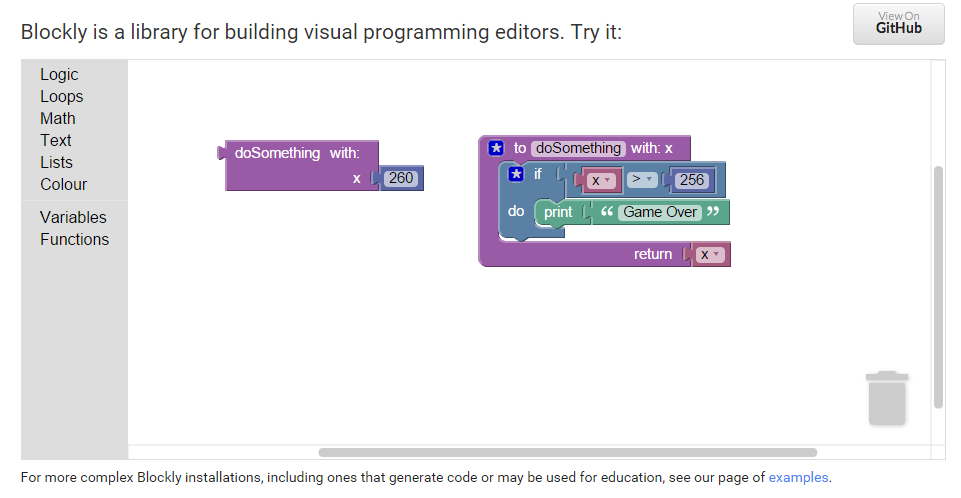
\includegraphics[width=1.2\textwidth]{./BestaandeSoftware/blockly.PNG}
\caption{Blockly.}
\end{figure}
\paragraph{Functies}
Blocky laat toe om functies te cree\"{e}ren. Functies kunnen parameters meekrijgen. Deze functies zijn globaal en kunnen vervolgens op elke plaats in het programma opgeroepen worden. Deze functies zijn gelijkaardig aan de functies van ons project. Echter behoren onze functies tot een bepaalde Klasse.
\paragraph{Operator Blokken}
Ons concept om operatoren toe te passen is gelijkaardig aan het concept dat Blockly gebruikt. Er is slechts 1 operator blok voor de binaire arithmische operatoren, alsook \'{e}\'{e}n operator blok voor de binaire logische vergelijkings operatoren. 
\begin{figure}[H]
\centering
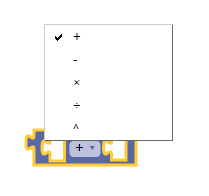
\includegraphics[width=0.4\textwidth]{./BestaandeSoftware/blocklyopp.PNG}
\caption{Blockly operators.}
\end{figure}
\subsubsection{Unreal Engine 4: Blueprints}
De Unreal Engine 4 \cite{unreal} is een game engine die uitgebracht is door Epic Games. In de Unreal Engine 4 is een visueel scripting systeem ingebouwd. Dit wordt Blueprints genoemd. Het laat toe om volledige gameplay elementen visueel te scripten via een node-based interface. Het is mogelijk om een volledige game te implementeren in Blueprints.
\begin{figure}[H]
\centering
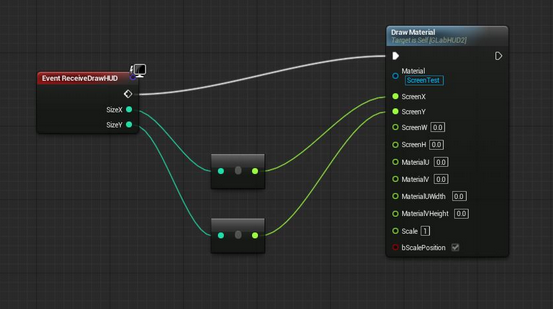
\includegraphics[width=1.1\textwidth]{./BestaandeSoftware/unrealEngine.PNG}
\caption{Unreal Engine 4.}
\end{figure}
De Unreal Engine gebruikt standaard enkel C++ code, ook voor de scripting. Blueprints compilen achterliggend ook naar C++ code. Hierdoor is er geen interpreting nodig van de nodes en is er ook geen snelheidsverlies.
\paragraph{Nodes}
In de Unreal Engine kunnen nodes verbonden worden met elkaar. Dit duidt op een opeenvolging, net zoals er in een imperatief programma de uitvoering van ene instructie overgaat naar de andere. Dit is te zien als de witte lijn. Vervolgens kunnen parameters doorgegeven worden, dit zijn de gekleurde lijnen. Dit kan vergeleken worden met ons systeem in het wireFrame. In ons systeem worden echter events met elkaar doorverbonden en niet de functies. \cite{unreal}
\paragraph{Events}
Het beginpunt van een flow van nodes in de Unreal Engine is een event dat ontvangen word. Dit kan een eigen gemaakt event zijn, of dit kan een standaard events zijn zoals te zien in de afbeelding.
\end{document}
\documentclass[]{article}
 
\begin{document}
 
\section{Diepgaande Beschrijving van het project}
\label{beschrijf}
 
\subsection{Diepgaande uitleg}
In deze sectie wordt op hoog niveau de IDE beschreven. Dit als korte inleiding voordat de algoritmes en datastructuren vermeld worden. Hierdoor kan verschillende terminologie verduidelijkt worden.\\\\
Zoals al eerder vermeldt kan een gebruiker de programma flow kunnen opbouwen in het deel van de IDE dat we het Frame-view noemen. Hierin kunnen instanties van klassen die eerder gedefineerd werden de mogelijkheid worden geboden om informatie aan elkaar door te geven. Deze informatie noemen we een Event. Wanneer een instantie een Event verstuurd en wat hij met een ontvangen Event doet is beschreven in de klasse waartoe hij behoort.\\\\ In de volgende paragrafen zal een diepgaande uitleg worden geven over wat een Events is en hoe de gebruiker er gebruik van maakt alsook hoe hij een klasse kan defini\"{e}ren en welke standaard eigenschappen een klasse in de IDE bevat.
\subsubsection{Events}
\label{Events}
Om onderlinge communicatie tussen Instanties van Klassen voor te stellen, gebruiken we een \textbf{Event}. Een Event kan al dan niet informatie bevatten. Een Event zonder informatie kan beschouwd worden als een trigger. De informatie dat een Event kan bevatten kan uit meerdere delen bestaan. De infomatie kan dus bestaan uit meerdere primitieve types (int, string of boolean). Elk deeltje in die informatie noemen we een variable. Met elke variable wordt een naam geassocieerd. Deze kan de gebruiker dan gebruiken om de variabele uit een Event op te vragen. Ook het Event zelf moet een ID hebben dat als type geldt.\\\\ Eens de gebruiker een Event heeft gedefineerd in de daarvoor voorziene omgeving kan hij er verder in de IDE gebruik van maken. Dit doet hij dan door deze Event te selecteren in een dropdown menu van bepaalde blokken, dit maakt een EventInstance aan. Hij kan dus vanaf dan een Event het eerder gedefineerde type aanmaken en invullen met de informatie die hij wenst mee te geven. 
Het zenden van een EventInstance door een klasse noemt een emit. Naar welke instanties van klassen het EventInstance wordt verzonden, kan worden bepaald in het Frame-view van de IDE.\\\\
\label{Visuele voorstelling: Frame-view van het canvas.}Er is een aparte view waarin alle Instanties van Klassen als blokjes getoond worden, dit view noemen we het \textbf{Frame-view}. Deze blokjes bevatten inkomende en uitgaande poorten. Deze stellen respectievelijk de evenementen voor die een Instantie wil ontvangen en de evenementen die het uitzendt. Er kunnen verbindingen gemaakt worden tussen de uitgaande poorten van een instantie en de inkomende poorten van een andere instantie, waarbij de respectievelijke evenementen hetzelfde type hebben.\\\\ 
Dit aparte view is echter de begin positie van alle gewenste Instanties van de aangemaakte Klassen. De gebruiker heeft de optie om de verbindingen al dan niet te tonen. Een extra view, het \textbf{Canvas-view} het bewegen van de instanties toont. De gebruiker kan zo de flow van Events bekijken.\\\\  
Nieuwe \textbf{Events kunnen aangemaakt worden} door de gebruiker in een aparte sectie van de IDE. Een Event moet een type hebben, vervolgens kan er informatie meegegeven worden aan dit Event. Deze informatie is een POD (plain old data) die opgebouwd wordt door de gebruiker. Hierin zal elke variable een unieke naam en specifiek type hebben. \\\\
Er zijn \textbf{standaard Events} beschikbaar zoals oa. KeyA, MousePress, Start, enz. Deze events zijn voorgedefineerd en dienen om interactie te hebben met het visuele canvas.  
\subsubsection{Klassen}
\label{Klassen}
Een Klasse kan worden vergeleken met eenderzijds een Sprite in de visuele programmeeromgeving Scratch \cite{scratch} en anderzijds een klasse uit een object ge\"{o}rienteerde taal zoals Java. Het verschil in deze applicatie is dat de Instanties van een Klasse expliciet aangemaakt worden in de Frame-view. Een Klasse bestaat uit: input Events, Handlers voor die Events, functie definities en member variabelen. Een Klasse kan worden voorgesteld in het Frame-view. Deze appearance kan door een functie in de Klasse worden veranderd. Een Instantie kan dan in het Frame-view beslissen van welke andere Instanties het die input Events ontvangt of naar welke instaties hij Events verstuurd. \\\\ Een Klasse kan \textbf{Events ontvangen}. Dit werd besproken \ref{Visuele voorstelling: Frame-view van het canvas.}. Het afhandelen van een Event gebeurt door een handler die het event binnen krijgt. Het raadplegen van de inhoud van een Event, kan doormiddel van een accessblok. Deze kan een variable accessen die in het binnenkomende event zit. \\\\Een Klasse kan \textbf{Events emitten}. Dit kan met behulp van een Emit blok. Hierin moet een Event worden geselecteerd. Als een Event informatie bevat zal deze ook hier moeten worden ingevuld. \\\\Een Klasse kan ook een overzicht hebben met alle Events die erdoor worden ge\"emit, dit is getoond in het Wire-view, indien een instance bestaat van die Klasse.\\\\Een uitbreiding van de visuele omgeving ten opzichte van andere IDE's is toe te laten om \textbf{functie aanroepen} te maken binnen een Klasse. Oorspronkelijk was het idee om dit voor te stellen met een lijn die twee functieblokken zou verbinden. Bij een Klasse met veel interne functie aanroepen wordt dit echter onoverzichtelijk.\\\\Een functie oproep vanuit een andere functie wordt voorgesteld door blokje. Dit blokje bevat de naam van de functie die kan worden opgeroepen. Alsook zijn input parameters en return waarde. De parameters worden by-value doorgegeven aan de functie. Hierin kunnen variable gebruikt worden die als constante worden doorgegeven. Een variable is data dat een bepaald type heeft zoals een number of string. Er kan geschreven worden naar een variable en de variable kan gelezen worden. De onderkant van een functieaanroep blok bevat een leeg vakje voor de return waarde. Hier kan een variabele aan gekoppeld worden om deze waarde op te vangen.\\\\\textbf{Member Variabelen} zijn variabele die gelden per Instantie van een Klasse. Deze kunnen bijvoorbeeld de toestand van van de Instantie van een Klasse die een lamp voorstelt in het canvas voorstellen.
 
\subsubsection{Blokken}
\label{primitive}
Een blok is een blokje dat de gebruiker kan plaatsen in het programmeer venster van de IDE. Deze blokken kunnen alles voorstellen, bv. variabelen, types, control-flow, functions, enz. . Deze zijn onderverdeeld in verschillende categorie\"en. De verdere uitleg met betrekking tot deze categorie\"en en de blokken die erbij horen staan in bijlage op Sectie~\ref{bijlageblok}.
 
 
\end{document}
\documentclass[]{article}

\begin{document}

\section{Evaluatiecriteria}
\label{EvaluatieCriteria}
Er zijn verschillende criteria die we stellen aan onze software. Sommige van deze criteria is subjectief en niet getoond in onderstaande bulletpoints. Onder de subjectieve criteria verstaan we oa. de professionele look van de IDE. 

\begin{itemize}
\item Multilanguage user interface (ondersteunde talen zijn engels en nederlands).
\item Geen crash bij inladen van foute XML data.
\item Verkeerde invoer onmogelijk maken bij het wireFrame (enkel events van hetzelfde type kunnen verbonden worden, en input kan enkel met output punten verbonden worden)
\item Het verzenden van events wordt gelijktijdig opgevangen door de geabonneerde instanties. De uitvoering van de code gebeurt hierna ook op een concurrent manier.
\item Mogelijkheid om projecten op te slaan.
\item IDE blijft niet vasthangen bij een infinite loop.
\item IDE geeft geen beperking op het aantal processes die tegelijkertijd kunnen runnen.
\item IDE geeft geen beperking op het aantal Klassen die tegelijkertijd kunnen bestaan.
\item IDE geeft geen beperking op het aantal Events die tegelijkertijd kunnen bestaan.
\item IDE geeft geen beperking op het aantal functions die tegelijkertijd kunnen bestaan.
\item Recursieve aanroepen zijn mogelijk.
\item Parameter passing is ge\"{i}mplementeerd.
\item Bij type-error op runtime breekt enkel dat proces af.
\item Bij variable-not-found error op runtime breekt enkel dat proces af.
\item Deadlocks zijn niet mogelijk d.m.v. de locks die de gebruiker kan gebruiker.
\item Er is geen probleem met racing conditions m.b.t. processen die dezelfde variabelen willen gebruiken indien de gebruiker locks gebruiker.
\item Processen worden in dezelfde orde toegevoegd als ze worden toegevoegd.
\item Geen globale variabelen.
\item Een lock kan niet gezet worden indien een ander proces al een lock gezet heeft op dezelfde instantie.

\end{itemize}
\end{document}
\documentclass[]{article}

\begin{document}
\section{Keuze programmeertaal: Java}
We hebben gekozen voor Java omwille van het grote aanbod van uitgebreide API's. Beide teamleden zijn bekend met de programmeertaal door de cursus object-geori\"{e}nteerd programmeren 2. Ook is de taal cross-platform wat een eis is van het project. Java biedt ook een sterke GUI libary aan nl. Swing.
\section{Algoritme en datastructuren}
\label{Algoritme}
Zoals al eerder vermeld in dit verslag is dient onze applicatie om event-driven programma's te maken. In de volgende sectie halen we kort aan wat het event-driven programming paradigma inhoudt en hoe we dit gaan implementeren. Verder halen we ook aan hoe we onze uitvoer gaan controlleren. Hier verkiezen we concurrent programming. We leggen onze keuze uit met voor en nadelen.
\subsection{Event-driven programming.}
Event-driven programming is een programmeer paradigma waarbij de flow van het programma wordt bepaald door events gecree\"{e}rd door de gebruiker zoals input events of door events veroorzaakt door delen in het programma \cite{eventdrivenwiki}.

\subsubsection{Extended handlers design pattern}
Als design pattern voor onze applicatie basseren we ons op het extended handlers design pattern dat Stephen Ferg uitlegt in zijn paper: Event-Driven Programming: Introduction, Tutorial, History \cite{eventdrivenStephen}.
\begin{figure}[H]
  \centering
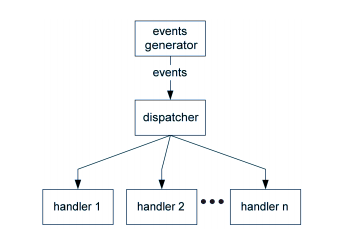
\includegraphics[scale=0.5]{AnalyseADTAlgorithm/extendedHandlerspattern.png}
  \caption{Extended handler.} \label{extendedHandler}
\end{figure}

In Figuur \ref{extendedHandler} stelt de eventgenerator in onze applicatie het generenen van events door gebruikers input en door instanties voor. Door dat events talrijk gegenereerd kunnen worden zal de Dispatcher een queue zijn die een stroom van events opvangt. Hij zal ervoor zorgen dat het event door de juiste handelers wordt afgewerkt.\\\\
Doordat in onze applicatie events worden doorgegeven aan specifieke andere instanties van Klassen zoals beschreven in de Sectie \ref{Events}. Zal de dispatcher ervoor moeten zorgen dat de juiste handlers van de juiste instanties worden aangeroepen.

\subsection{Concurrent computing }
Concurrent computing \cite{concurrent} is een vorm van computing waarbij een deel berekeningen worden uitgevoerd zodat het lijkt alsof ze gelijktijdig worden uitgevoerd. We hebben ervoor gekozen om niet multi-threaded te werken om de complexiteit van het project zo laag mogelijk te houden.\\\\ Daarom is concurrent computing de oplossing voor onze applicatie. In tegenstelling tot parallel computing is dit wel mogelijk op een thread. Gelijktijdige processen zoals twee events die samen worden opgeroepen lijken hierdoor ook gelijk te worden afgehandeld. In tegenstelling tot het sequentiel uitvoeren van de twee events.\\\\
Bij concurrent computing worden processen in executie stappen opgedeeld. Er wordt gebruik gemaakt van timeslices waarin van elk proces een deel executie stappen worden uitgevoerd, wij noemen dit een primitieve stap. Na dat bepaald aantal of tijd wordt het proces gepauzeerd en verder gegaan met het volgende. Dit wordt herhaald zolang een proces niet volledig is afgerond.
\subsubsection{Verschil met parallel computing}
Parallel computing is gelijkaardig aan concurrent computing, echter gebeurt het werk op verschillende cores. Bij concurrent computing zal de uitvoering van twee identieke events die gelijktijdig worden aangeroepen niet gelijktijdig eindigen omdat de uitvoering steeds wisselt tussen de twee events. 

\subsubsection{Probleem met concurrent computing}
Een eerste probleem is racing conditions. Hierbij proberen twee processen hetzelfde algortime uit te voeren waarbij een bepaalde sequentie van uitvoering belangrijk is. Het volgende voorbeeld gevonden op \cite{concurrent} toont een functie waarbij een private member variabele balance wordt geaccessed en verandered. Stel dat er twee processen runnen die respectievelijk withdraw(200) en withdraw(300) oproepen en dat balance 250 bedraagt. Bij beide processen zal de conditie 250 $>$ withdrawal, slagen, want balance is nog niet aangepast. Echter zal hierna balance aangepast worden en uiteindelijk -250 bedragen. Dit is een verkeerde uitvoering.
\lstset{language=Java}
\begin{lstlisting}
public class Main {
	public boolean withdraw(int withdrawal) {
    	if (balance >= withdrawal) {
        	balance -= withdrawal;
        	return true;
    	}	 
    	return false;
	}
}
\end{lstlisting}
Onze oplossing hiervoor is een lock op een private member variabele toelaten. Deze zorgt dan dat enkel dat proces aan die variabele kan voor zowel te lezen als te schrijving.\\\\
Hierbij komt een ander probleem tevoorschijn, nl. een deadlock \cite{deadlock}. Om dit probleem op te lossen stellen we dat slechts \'{e}\'{e}n proces gelijktijdig locks kan aanbrengen.

\subsection{Drawing}
\paragraph{Blokken}worden getekend door middel van rechthoeken. Deze kunnen genest worden in elkaar.
\paragraph{Het WireFrame}is de collectie van Instances en Wires. Een Instance wordt getekend als een blok waarop enkele punten getekend zijn die de inkomende en uitgaande Events voorstellen. De Wires worden getekend als lijnen. Deze lijn kan bestaan uit meerdere punten en wordt getekend door de gebruiker. Deze lijn zal dus niet automatisch gegenereerd worden.

\subsection{Model en Controller}
Elke visuele component is verbonden met een model (zie Sectie \ref{ModelBlock}). Dit model bevat info die nodig is om aan type checking te doen in de GUI. Ook worden de blokken die genest zitten in deze blok bijgehouden in het model. De wireFrame zal ook voorgesteld worden als een Model. De controller die behoort tot een model zal nagaan of een blok genest kan worden in een bestaande blok door informatie op te vragen aan het model van de bestaande block. Er wordt ook doorgegeven wanneer er iets genest wordt.

\subsection{Runtime}
\label{Runtime}
Op het hoogste niveau is een Runtime (zie Sectie \ref{runtimeClass}) aanwezig. De IDE gebruikt een Abstracte klasse Runtime zodanig dat de gebruikte programmeertaal niet direct vasthangt aan de IDE. Er is een klasse aanwezig die de Runtime voor de ge\"{i}mplementeerde programmeertaal implementeerd. De abstracte Runtime bevat alle modellen van de blocks alsook het wireFrame model, de ge\"{i}mplementeerde Runtime bevat de nodige data voor de executie van de code zoals een Compiler en een Virtual Machine (zie Sectie \ref{VM}). De Runtime zorgt voor de vlotte uitvoering van alle code. Er is een functie aanwezig die continue de Virtual Machine aanroept zolang er niet gestopt moet worden. Door een aparte thread aan te maken zal hij deze functie parallel kunnen runnen met de GUI. Verdere executie is uitgelegd in Sectie \ref{VM}.

\subsection{Compileren}
\label{Compileer}
Elke visuele view van een blok heeft een model zoals uitgelegd. Deze blok wordt bij het compileren meegegeven aan een Compiler Klasse door de Runtime. Deze klasse is een information expert met betrekking tot compileren. De IDE gebruikt een Interface Compiler zodanig dat de gebruikte programmeertaal niet direct vasthangt aan de IDE. Hij heeft verschillende functies die elk een ander type BlockModel (\ref{ModelBlock}) compileren. Omdat het wireFrame ook voorgesteld wordt als een model kan het wireFrame simpel gecompileerd worden omwille van deze functies. Elk model weet welke blokken genest zijn zullen alle geneste blokken ook worden gecompileerd. Het design van de Compiler is het visitor design pattern. Het algoritme voor het compilen van een blok wordt gescheiden van de datastructuur van de blok.  

\subsection{Virtual Machine}
\label{VM}
Onze virtual machine bevat een lijst van alle processen die momenteel moet uitgevoerd worden. Incrementeel zal er telkens \'{e}\'{e}n  primitieve stap uitgevoerd worden van elk proces. Als er een proces uitgevoerd moet worden, zal dit toegevoegd worden aan het einde van de lijst. Als een bepaald proces klaar is, wordt dit verwijderd uit de lijst. \\\\
Als een Event verstuurd wordt zal de Virtual Machine dit Event doorgeven aan een Event Dispatcher. Dit is een Klasse die de taak voor het verzenden van Events op zich neemt. De Event Dispatcher kent alle verbindingen tussen de Instanties, en hiermee kunnen nieuwe processen aangemaakt worden zodat de Virtual Machine deze kan gebruiken. 
\subsubsection{Een proces}
Een proces (zie Sectie \ref{procesklass}) is een gesimuleerde thread. Deze beheert nodige data zoals een variable-stack en code. Een proces wordt uitgevoerd door de VM. Een proces kan gerunned worden en deze zal dan \'{e}\'{e}n primitieve stap \ref{primitive}uitvoeren.
\subsubsection{Stoppen van uitvoering}
Voor het stoppen van de uitvoer zal er een event worden verzonden naar de Runtime bij het opvangen van dit event zal de uitvoering worden gestopt.

\subsection{Voorbeeld implementatie}
\label{voorbeeldvm}
Er bestaat een Klasse die een input event: event1 accepteerd. Dit event wordt afgehandeld door handler1 van de Klasse. De gebruiker heeft deze handler ge\"{i}mplementeerd in blokken op de volgende manier:
\lstset{language=Java}
\begin{lstlisting}
Event event1{
	members:
		- member1(number, value)
}
class Class1 {

	handler( event1) {
    		makeVar(number, x)
    		set(X, acces(event1, member1)
    		functieCall(functie1, parameters: x, return:x)
	}
	
	functie(functie1, parameters: z){
		while(z < 10){
		set(z, z + 1)
		}
		return z;
			
	}
	
	
}
\end{lstlisting}
Instantie instance1 is een instantie van Class1 waarnaar een instantie van event1 wordt verzonden. De eventDispatcher zal dus een proces aanmaken met instantie1 en op de Code stack de handler pushen.\\
Het uitvoeren van het proces zal in de volgende primitieve stappen gebeuren:\\\\
\textbf{Stap 1:} De handler zal zijn execute functie uivoeren. Deze zal een nieuw FunctieFrame aanmaken. Ook zal de eventInstance die mee werd gegeven bij het aanmaken van het proces op de stackframe geduwd. De blok van de handler op de Stack wordt vervangen door de inhoud.\\
\textbf{Stap 2:} De execute van makeVar zal een nieuwe variable van het type number maken op het huidige FunctieFrame.\\
\textbf{Stap 3:} De execute van Set zal de het Event in de huidige Stackframe zoeken en hieruit de juiste member halen nl. member1. De waarde hiervan wordt in x geplaatst. We gaan er van uit dat member1 $=$ 8.\\
\textbf{Stap 4:} De execute van FunctieCall doet de volgende stappen. Ophalen van de de parameter waarde die in de call staan. Deze slaat gij op in volgorde van de oproep. Hierna haalt hij het functieblok met de juiste functie naam op. Hiervan haalt hij de parameter namen op. Hij cree\"{}ert een nieuw FunctieFrame en daarop pushed hij de parameternamen met de juiste eerder opgehaalde waarde. Hier is dit dus z met de waarde 8. Dit gebeurt achter de schermen met makeVar- en set-blokken. Hierna worden er eerst nog set-blokken voor de return waardes op de stack gepushed. Nu wordt de execute van de functie aangeroepen. Deze zal al zijn blokken op de stack pushen zonder nieuw frame te cree\"{e}ren.\\
\textbf{Stap 5:} De bovenste blok is nu de While blok. De execute van deze blok zal zijn conditie controleren nl $z < 10$ deze evalueert naar true aangezien x $=$ 8. Hierdoor zal de body van de While-blok op de code stack worden gepushed. Maar eerst wordt de While-blok er zelf ook nog op gepusht.\\
\textbf{Stap 6:} De waarde van X wordt in de set-blok verhoogt met 1.\\
\textbf{Stap 7:} herhaling stap 5.\\
\textbf{Stap 8:} herhaling stap 6.\\
\textbf{Stap 9:} De conditie van de While-blok evalueert nu naar false. Hierdoor worden er geen blokken op de code stack gepusht.\\
\textbf{Stap 10:} De return blok zoekt in de huidige FunctieFrame de waarde van z op en plaats deze in de returnVariables.\\
\textbf{Stap 11:} Aangezien de functie is afgelopen mag het FunctieFrame van de stack worden gepopt.\\
\textbf{Stap 12:} De set-blok zal nu x in het huidige FunctieFrame veranderen naar de return waarde\\
\textbf{Stap 13:} Het proces bevat geen blokken meer dus zal een ProcesFinishedException gooien naar de VM deze zal het proces verwijderen uit de queue.
 
\begin{figure}[H]
\centering
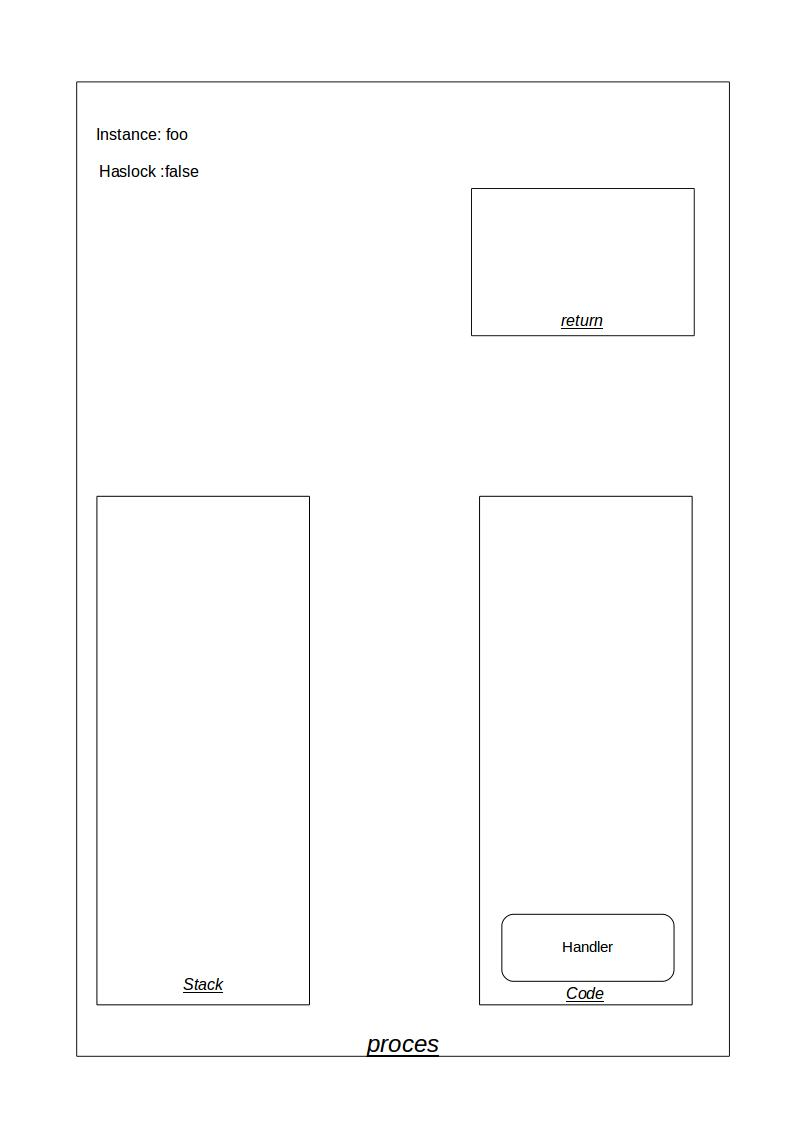
\includegraphics[scale=0.4]{AnalyseADTAlgorithm/processtappen/stap1.jpg}
\caption{Stap 1}
\end{figure}

\begin{figure}[H]
\centering
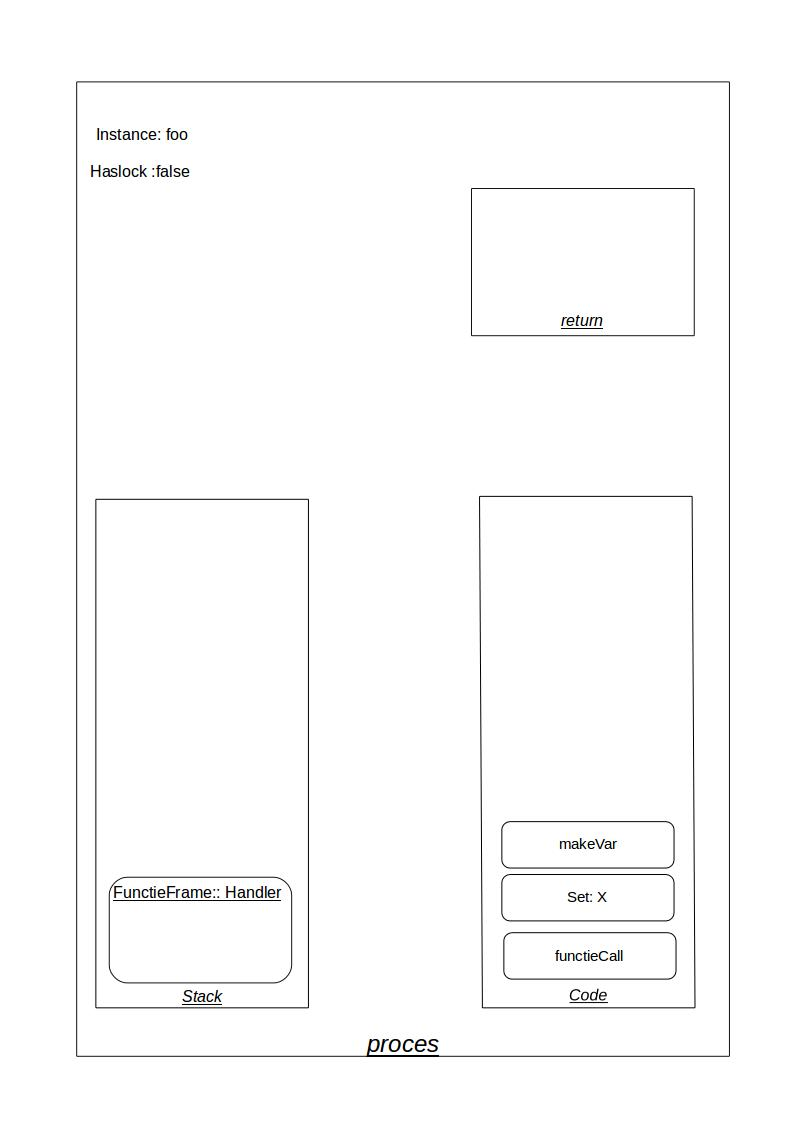
\includegraphics[scale=0.4]{AnalyseADTAlgorithm/processtappen/stap2.jpg}
\caption{Stap 2}
\end{figure}

\begin{figure}[H]
\centering
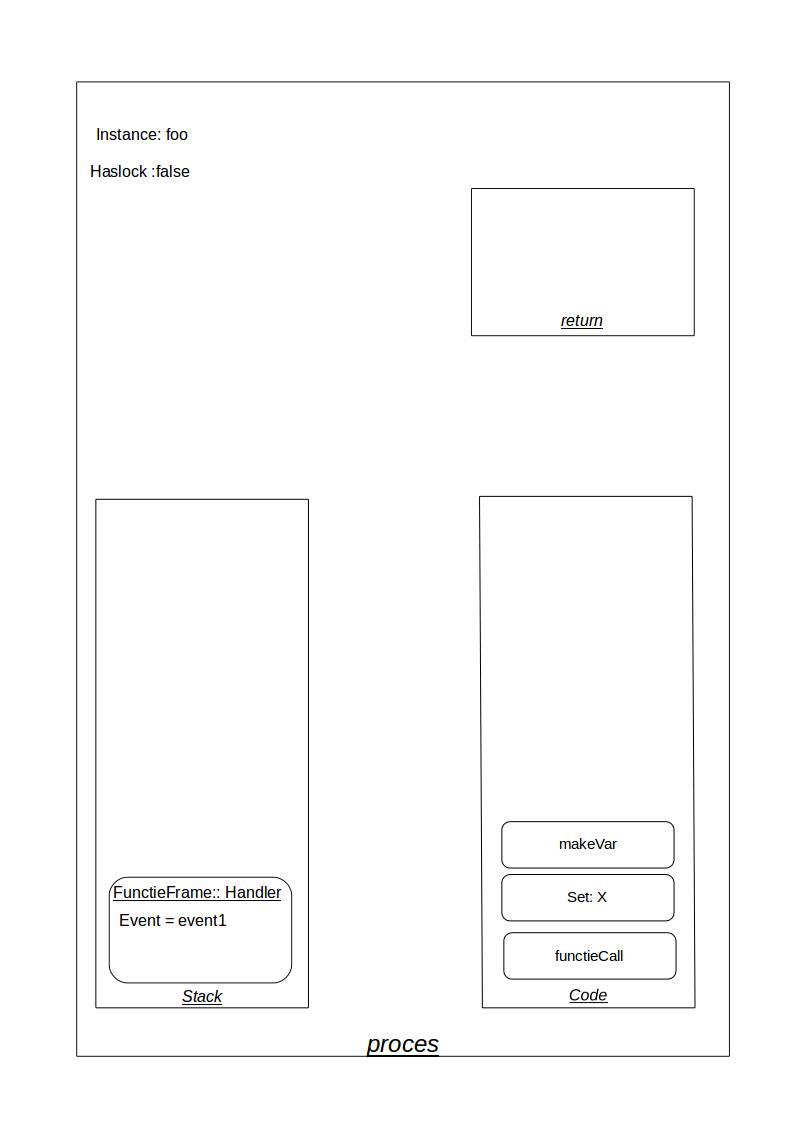
\includegraphics[scale=0.4]{AnalyseADTAlgorithm/processtappen/stap3.jpg}
\caption{Stap 3}
\end{figure}
\begin{figure}[H]
\centering
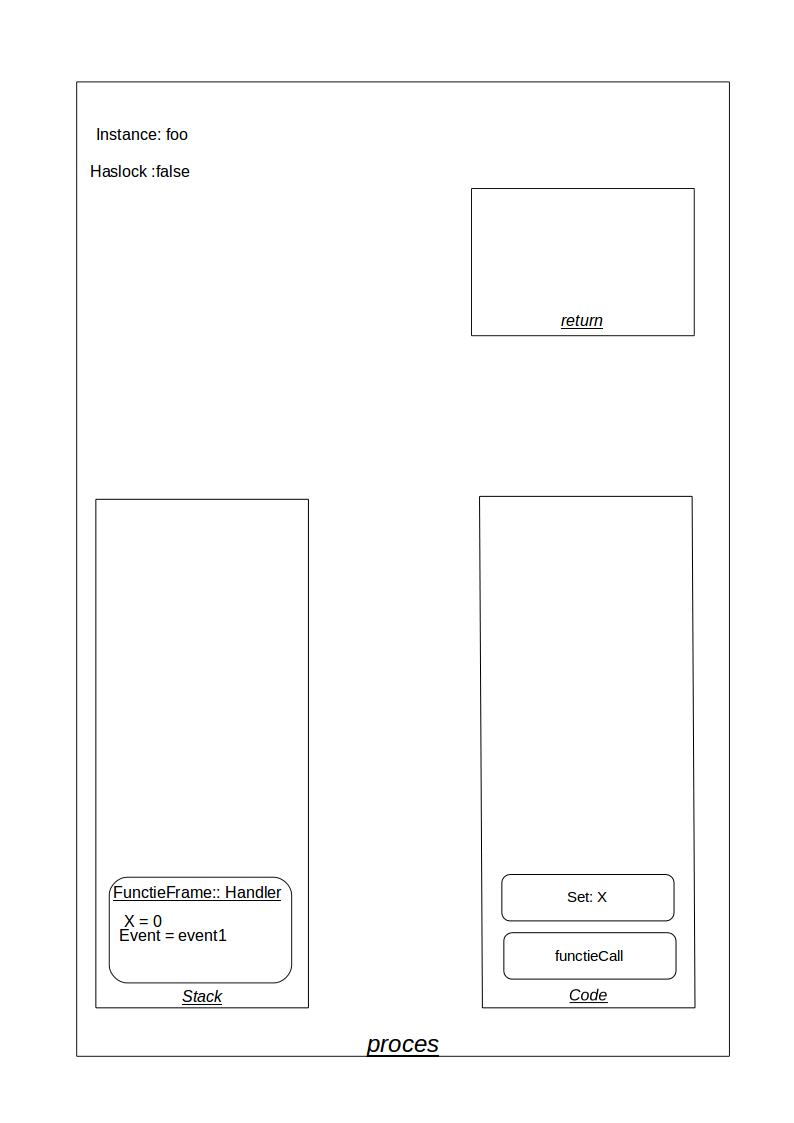
\includegraphics[scale=0.4]{AnalyseADTAlgorithm/processtappen/stap4.jpg}
\caption{Stap 4}
\end{figure}
\begin{figure}[H]
\centering
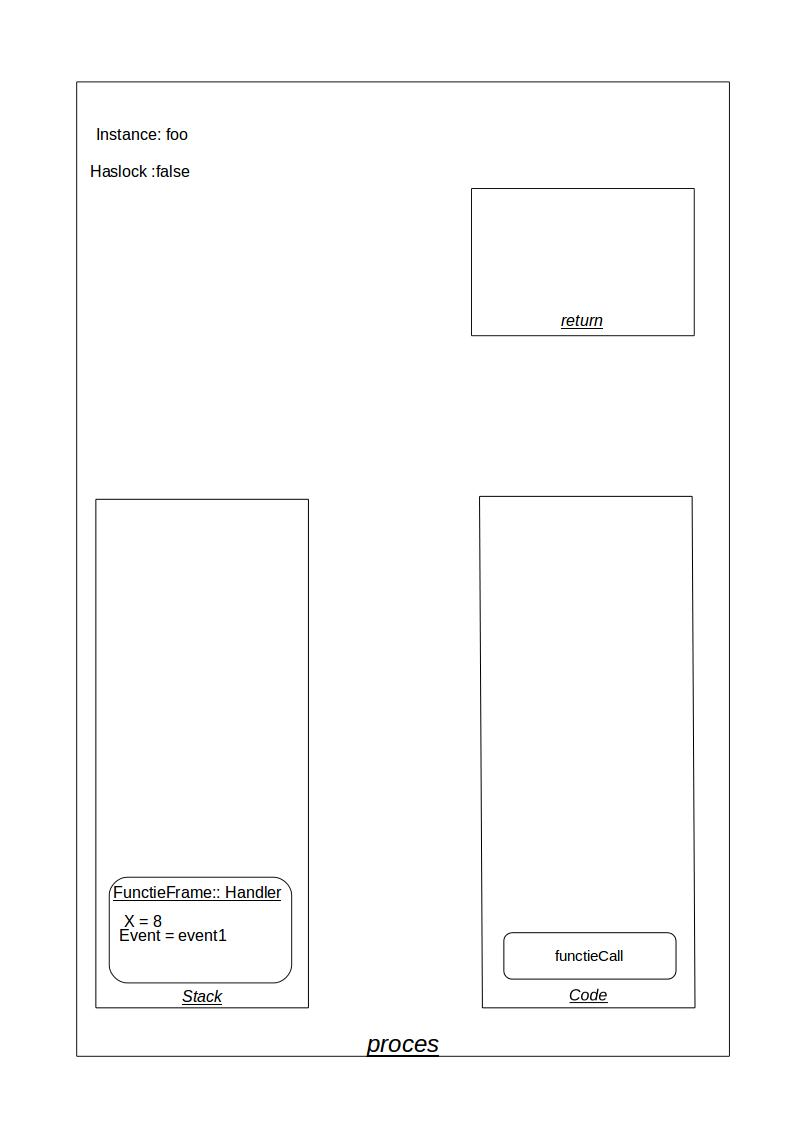
\includegraphics[scale=0.4]{AnalyseADTAlgorithm/processtappen/stap5.jpg}
\caption{Stap 5}
\end{figure}

\begin{figure}[H]
\centering
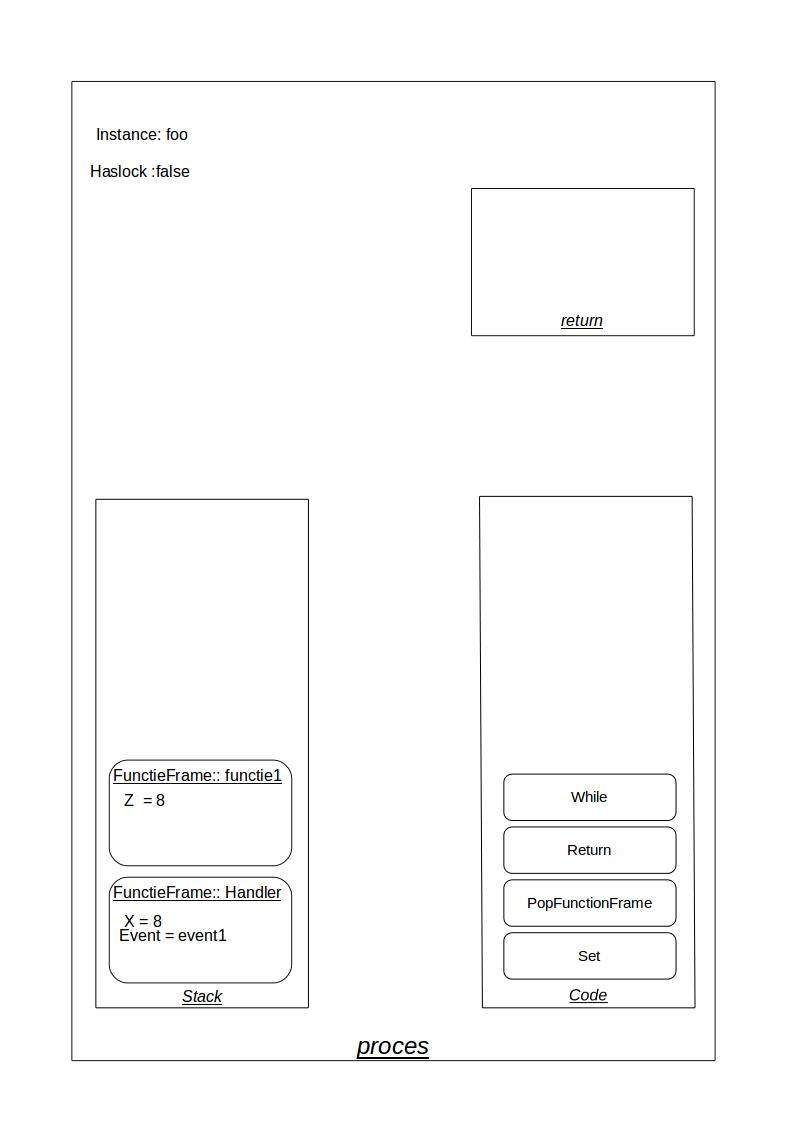
\includegraphics[scale=0.4]{AnalyseADTAlgorithm/processtappen/stap6.jpg}
\caption{Stap 6}
\end{figure}

\begin{figure}[H]
\centering
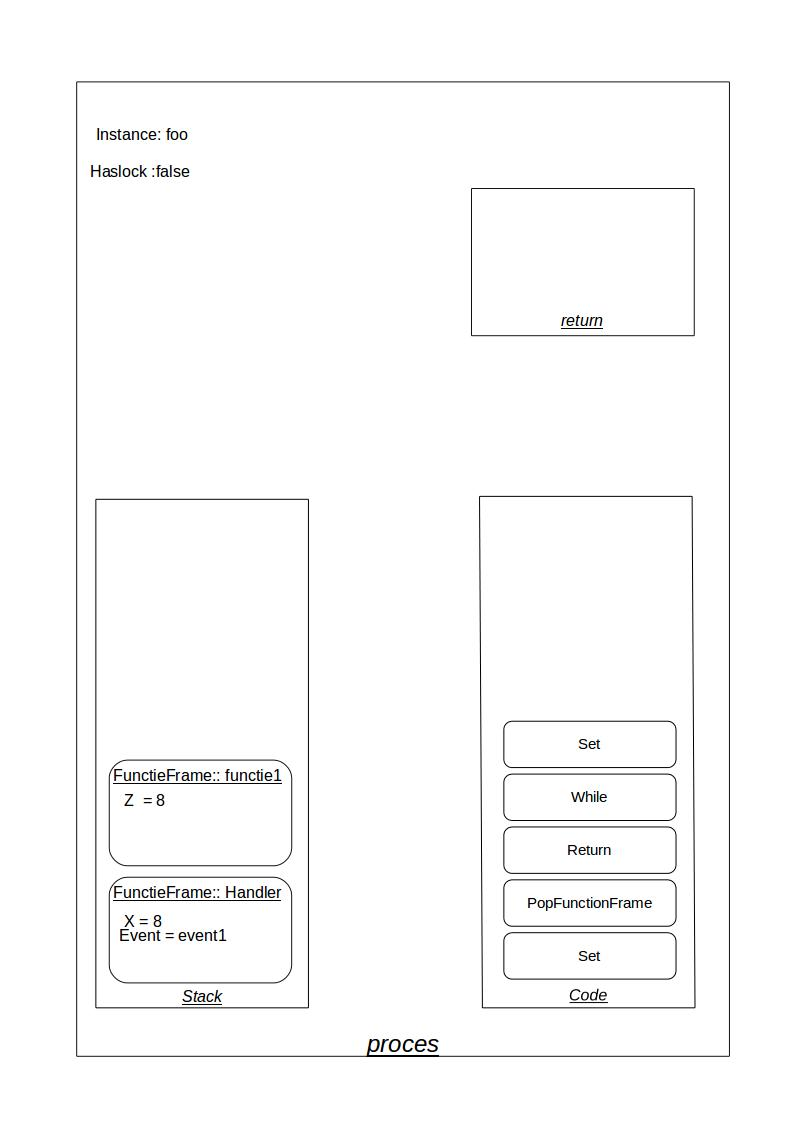
\includegraphics[scale=0.4]{AnalyseADTAlgorithm/processtappen/stap7.jpg}
\caption{Stap 9}
\end{figure}

\begin{figure}[H]
\centering
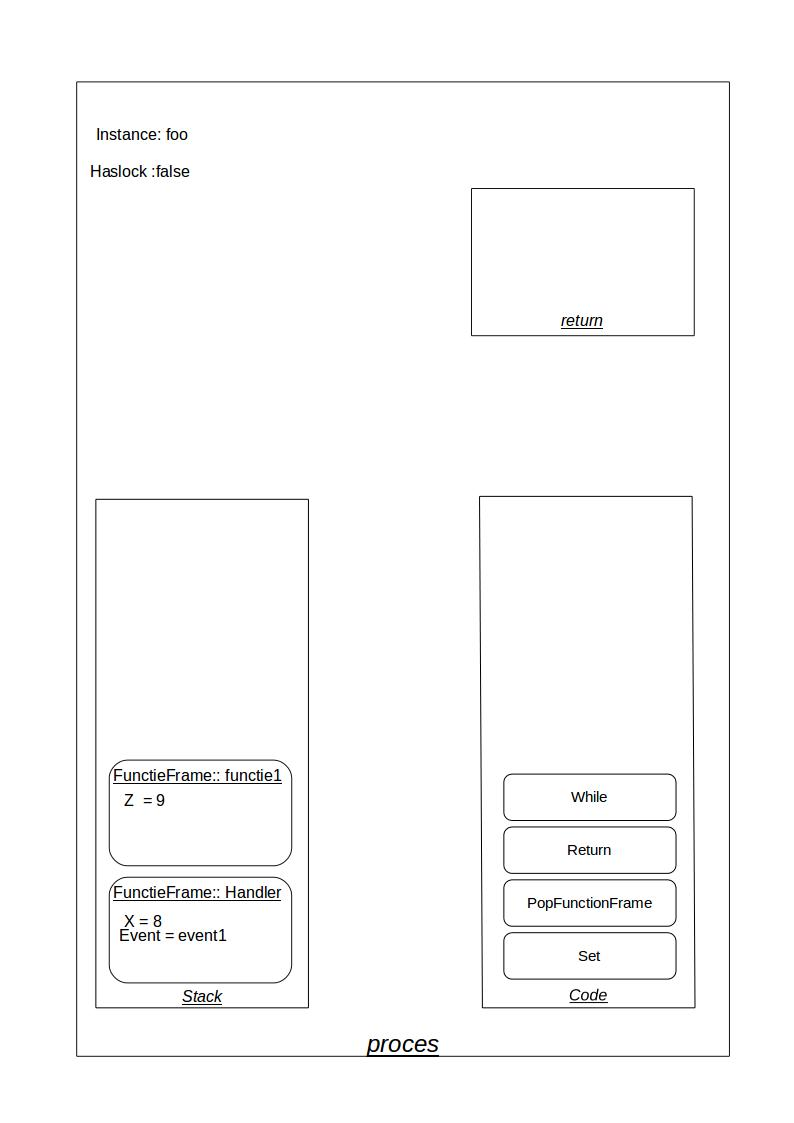
\includegraphics[scale=0.4]{AnalyseADTAlgorithm/processtappen/stap8.jpg}
\caption{Stap 10}
\end{figure}

\begin{figure}[H]
\centering
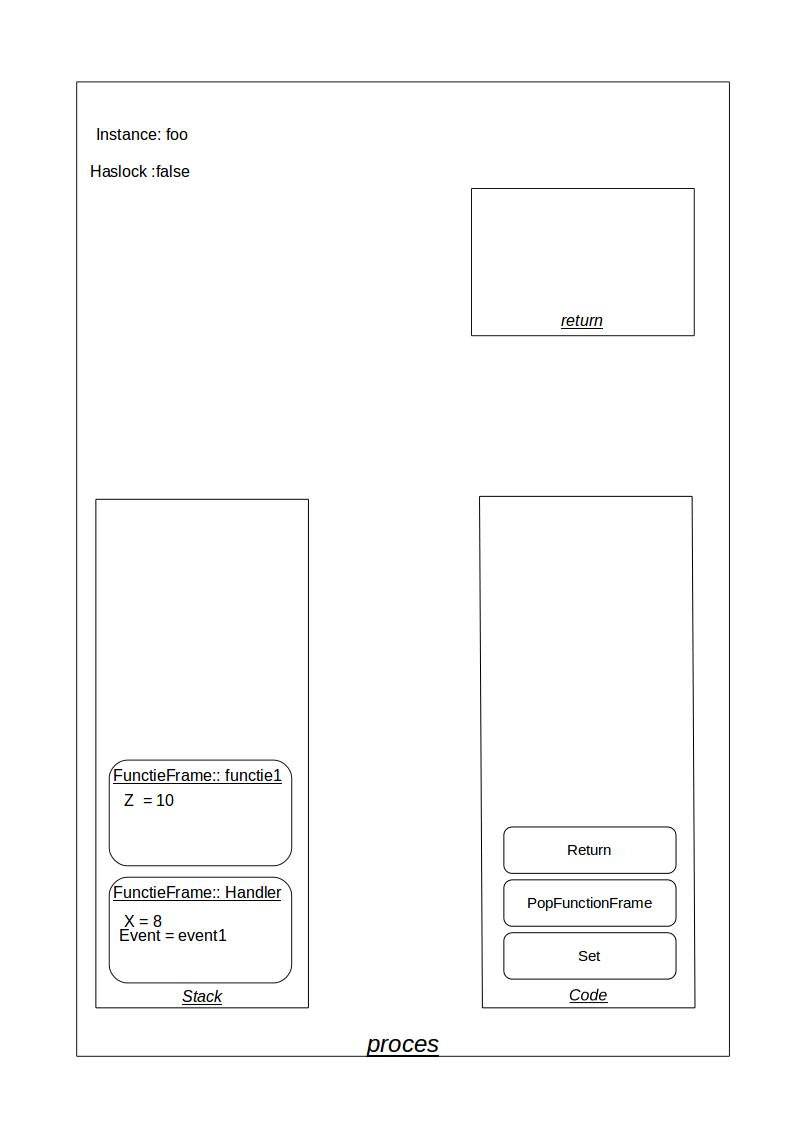
\includegraphics[scale=0.4]{AnalyseADTAlgorithm/processtappen/stap9.jpg}
\caption{Stap 11}
\end{figure}
\begin{figure}[H]
\centering
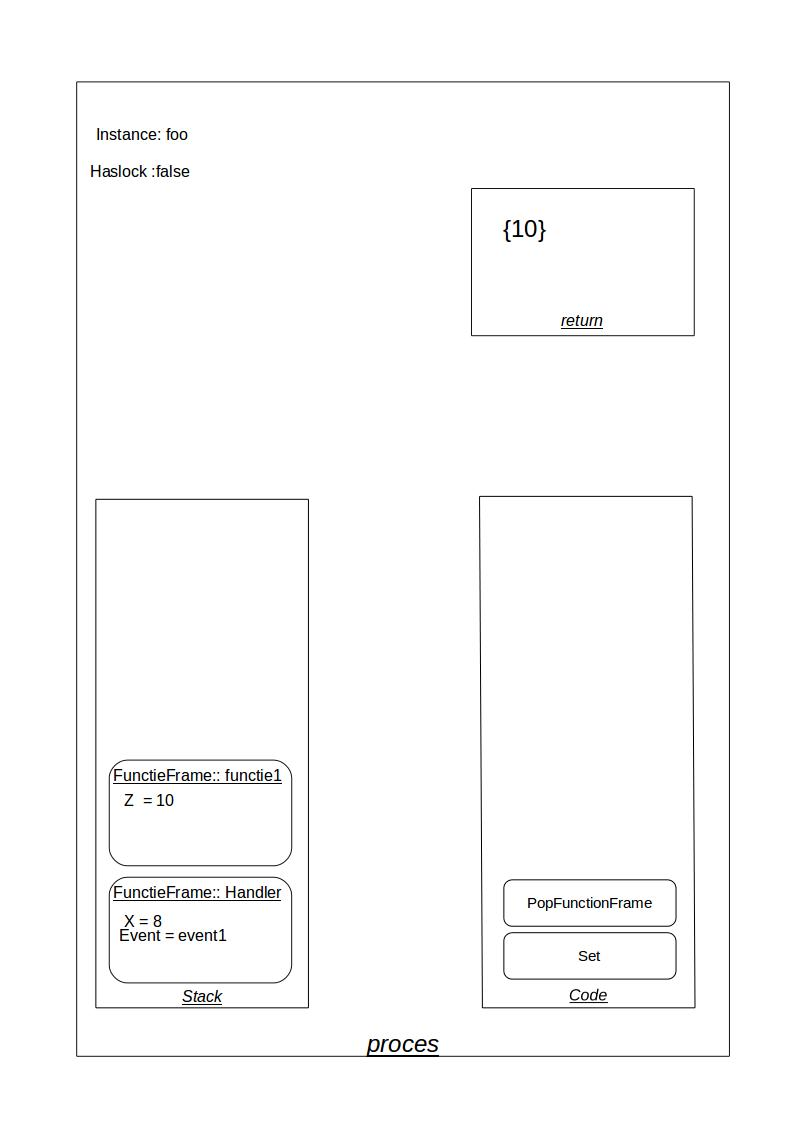
\includegraphics[scale=0.4]{AnalyseADTAlgorithm/processtappen/stap10.jpg}
\caption{Stap 12}
\end{figure}
\begin{figure}[H]
\centering
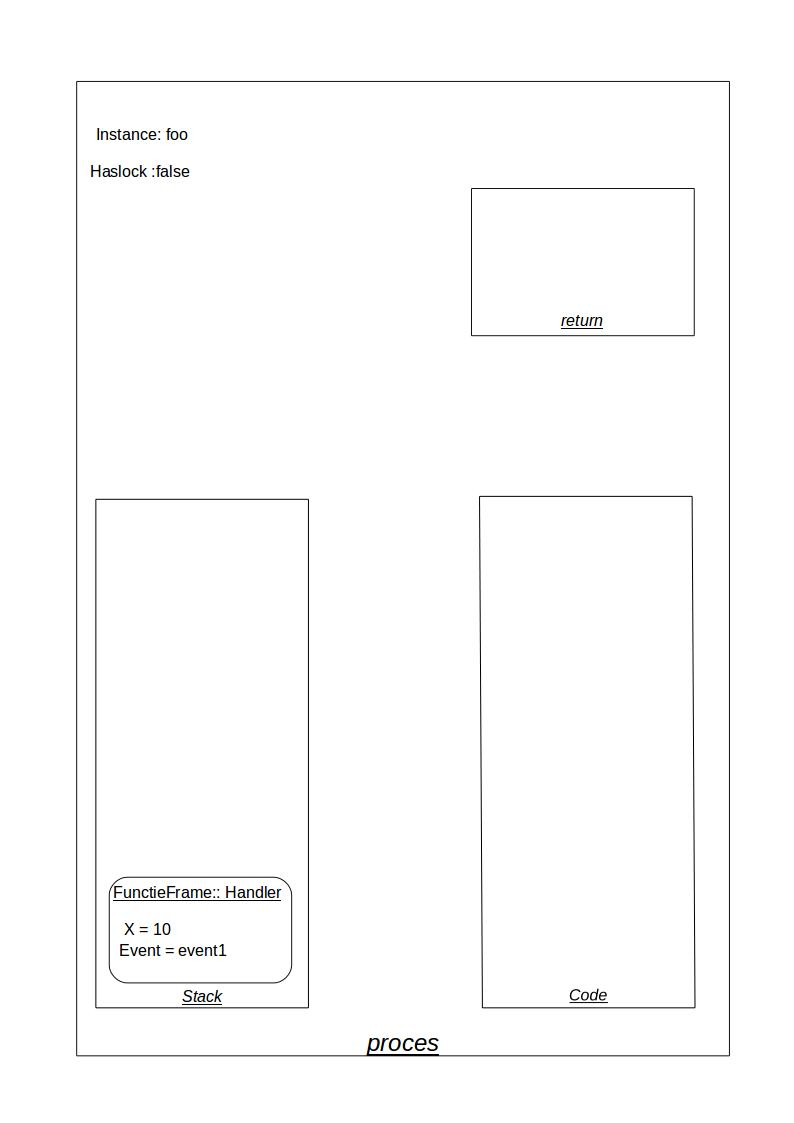
\includegraphics[scale=0.4]{AnalyseADTAlgorithm/processtappen/stap11.jpg}
\caption{Stap 13}
\end{figure}

\subsection{Lambda expressions}
\label{lambda}
Sinds 1.8 biedt java de mogelijk aan om lambda expressions \cite{lambda} te gebruiken, we gaan hier dan ook gebruik van maken. Onze operator blok is hier geschikt voor. Via lambda expressions kan men anonieme interface methodes aanmaken. Hieronder volgt een voorbeeld waarin duidelijk volgt hoe wij het zouden gebruiken. 
\lstset{language=Java}
\begin{lstlisting}
public class Calculator {
  
    interface IntegerMath {
        int operation(int a, int b);   
    }
  
    public int operateBinary(int a, int b, IntegerMath op) {
        return op.operation(a, b);
    }
 
    public static void main(String... args) {
    
        Calculator myApp = new Calculator();
        IntegerMath addition = (a, b) -> a + b;
        IntegerMath subtraction = (a, b) -> a - b;
        System.out.println("40 + 2 = " +
            myApp.operateBinary(40, 2, addition));
        System.out.println("20 - 10 = " +
            myApp.operateBinary(20, 10, subtraction));    
    }
}
\end{lstlisting}
In de operator block zal een statische hashmap bijgehouden worden. Deze word slechts \'{e}\'{e}n keer ge\"{i}nitialiseerd. In deze hashmap worden strings gemapt op lambda functies. De string $+$ mapt op een lambda functie enz. Deze lambda functie wordt hieronder beschreven:
\begin{lstlisting}
    interface OperatorMath {
        Variable operation(Variable a, Variable b);   
    }
  
    OperatorMath addition = (a, b) -> a.addVar(b);
    OperatorMath subtraction = (a, b) -> a.subVar(b);
\end{lstlisting}
\section{Code structuur}
Alle code zal opgedeeld worden in verschillende modules. Deze modules defini\"{e}ren hoe er met andere modules gecommuniceerd word. Hierdoor word het gemakkelijk om modules intern van werking te veranderen zonder dat er iets moet veranderen aan andere modules. Een module is een cluster van klassen die instaan voor elk instaan voor een doel dat beschouwd wordt door de module.

\subsection{Exceptions Module}
\label{ExceptionsModule}
Deze module heeft enkel als verantwoordelijkheid om alle excepties te groeperen.

\subsection{Variables Module}
\label{VariablesModule}
Deze module bevat alle klassen die te maken hebben met de data types die gebruikt worden.

\subsection{Blocks Module}
\label{BlocksModule}
Deze module implementeerd alle executie bloks die aanwezig zijn in de IDE.

\subsection{Collections Module}
\label{CollectionsModule}
Deze module bevat klasses die higher level zijn dan blocks. Het zijn collecties van Events, Classes, Instances.

\subsection{Core module}
\label{CoreModule}
Deze module staat in voor het uitvoeren van de code. De output van de compile module \ref{compile} zal door de VM module uitgevoert worden. Deze module kan werken in een release mode waarbij code normaal uitgevoert word, of in een debug modus waarbij er stap voor stap doorgeen het programma gelopen kan worden. 

\subsection{Model module}
\label{ModelModule}
Deze module is de representatie van alle code die gemaakt kan worden in de visuele IDE. Deze module zal ook instaan voor het nakijken van de code op syntax fouten (zie Sectie \ref{ModelBlock}). Deze module heeft verschillende klassen om events, Klassen, instances, variabelen en primitieve code blokken voor te stellen. 

\subsection{Runtime module}
\label{RuntimeModule}
\label{compile}
Deze module zal instaan voor het compilen en runnen van de code. De module zal een bepaalde hoeveelheid ruwe code van Klassen, Instances en Events omvormen naar uitvoerbare code. Deze module bevat ook een klasse die de runtime regelt van de programmeertaal van de IDE.

\subsection{File module}
Deze module behandeld het laden en saven van de IDE data. Deze data omvat de XML data. Er wordt ook gezorgd voor het multilanguage maken van de applicatie (zie Sectie \ref{Multilanguage}).

\subsection{GUI}
De GUI wordt momenteel bekeken als \'{e}\'{e}n grote module maar zal nog opgedeeld worden in kleinere modules zoals een menu module, etc. 



\end{document}
\documentclass[]{article}
 
\begin{document}
\section{Klassen per module}
Hierin worden alle grote klassen beschreven per module die gebruikt worden in de IDE. Elke klasse wordt kort toegelicht over hun functie, welke ADT's gebruikt hebben alsook hoe alle klassen samenwerken.

\subsection{Exceptions}
De verantwoordelijkheden van deze module worden beschreven in Sectie \ref{ExceptionsModule}.
\subsubsection{TypeException}
Deze wordt opgeroepen als er op runtime een type error gebeurt. De uitvoer van het uitvoerend proces wordt dan gestopt. De andere blijven doorgaan.
\subsubsection{ProcesFinishedException}
Deze exception wordt opgeroepen als een proces geen blocks meer bevat om uit te voeren.
\subsubsection{LockedException}
Deze Exception wordt opgeroepen als er een member variable van een Instance wordt aangesproken die gelocked is.
\subsubsection{OutOfBoundsException}
Deze exception wordt opgeroepen in CharAtBlock als in foute index wordt meegegeven.

\clearpage
 \begin{sidewaysfigure}
  \centering
   
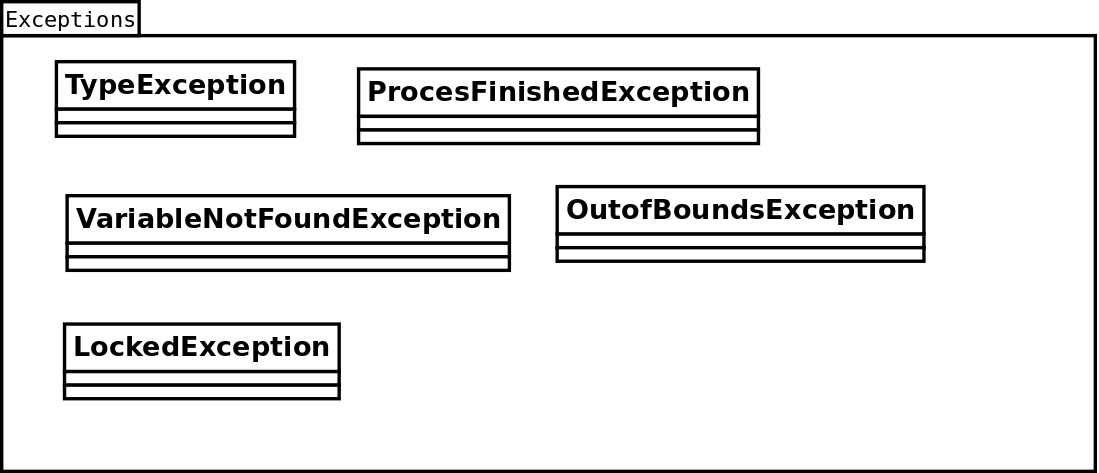
\includegraphics[scale=0.8]{./AnalyseClassenDiagram/exceptions.png}
  \caption{Exceptions Module.} \label{exceptionUML}
\end{sidewaysfigure}
\clearpage

\subsection{Variables}
De verantwoordelijkheden van deze module worden beschreven in Sectie \ref{VariablesModule}.
\subsubsection{EventInstance}
Een event bevat een Event voor zijn type Event waarvan het een instance is bij te houden en een Hashmap \cite{hashmap} waarbij het de naam van een variable (String) mapt op een variabele.
\subsubsection{ReturnVariables}
De ReturnVariables is klasse die gebruikt om return values in op te slaan en terug aan de functioncall. Deze bevat een stack \cite{stack} waarop de return waarde worden geduwt. Op deze manier kunnen we meerdere return values mogelijk maken. Echter voorzien we eerst maar een return value.
\subsubsection{Type}
\label{Type}
Dit is Enumeratie die een van de volgende kan zijn: Boolean, String, Number, Event of Value. Een value is een letterlijke inputwaarde door de gebruiker. Deze is nog niet geconverteerd naar een feitelijk type en kan dus eenderwelk type voorstellen.
\subsubsection{Abstact Class Variable}
\label{variable}
Deze klasse stelt een variabele voor. Deze heeft een Type als member.
\subsubsection{BooleanVariable}
Deze wordt afgeleid van de Abstact Class Variable en bevat dus een boolean als variable.
\subsubsection{NumberVariable}
Deze wordt afgeleid van de Abstact Class Variable en bevat dus een number als variable.
\subsubsection{StringVariable}
Deze wordt afgeleid van de Abstact Class Variable en bevat dus een String als variable.

\clearpage
 \begin{sidewaysfigure}
  \centering
   
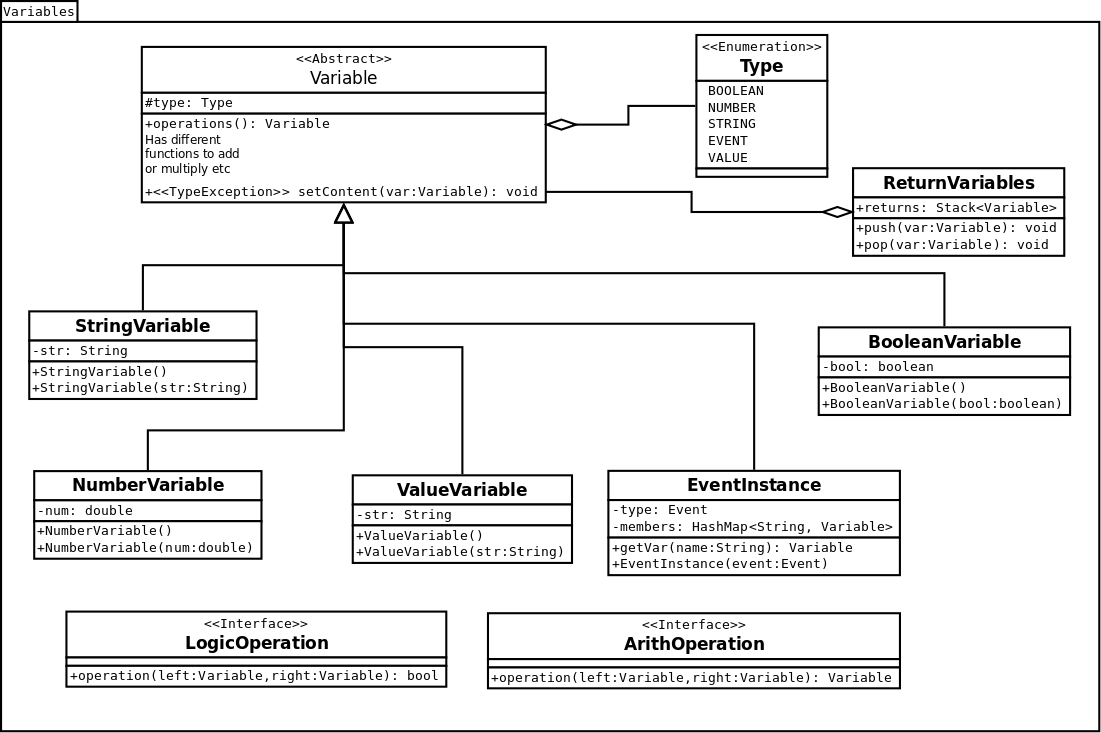
\includegraphics[scale=0.8]{./AnalyseClassenDiagram/variables.png}
  \caption{Variables Module.}
\end{sidewaysfigure}
\clearpage

\subsection{Blocks}
De verantwoordelijkheden van deze module worden beschreven in Sectie \ref{BlocksModule}.
\subsubsection{De Interface Block}
Een Block stelt een klasse voor die een bepaald stuk code voorstelt. Deze bevat een execute functie die een proces meekrijgt zodat hij zijn code kan uitvoeren of plaaten op het proces.
\subsubsection{HandlerBlock}
Deze implementeert de interface Block. Deze bevat een \texttt{ArrayList<Block>} \cite{arraylist} die we de body noemen. De heeft een EventInstance die hij mee kreeg op oproep, via zijn constructor. Deze wordt mee op zijn variabele stack gepushed bij het aanmaken van zijn FunctionFrame. De execute van deze block pushed de body als individuele blokken op de stack van het proces dat hij meekrijgt. Achteraan de body plakt hij nog een PopBlock.
\subsubsection{PopBlock}
Deze implementeert de interface Block. De execute van deze Block popt het bovenste FunctionFrame van de stack van het proces.
\subsubsection{AccessBlock}
 Deze bevat twee Strings namelijk de naam van het EventInstance waarvan het een member wil opvragen. En de naam van die member. De execute functie zal dus het EventInstance van de FunctionFrame opvragen. Hierin vraagt hij de variable op van de member en deze geeft hij terug.
\subsubsection{BroadCastBlock}
Bevat een naam van het Event. En een Hashmap \cite{hashmap} van Strings die de members van het event voorstellen deze worden gemapt op Blocks. De execute van dit Block zal deze Blocks uitvoeren en de bekomen variabele kopieren en mappen op de juiste string. Het zal dan een aangemaakte event terug geven aan het proces. Dat dit op zijn beurt doorgeeft aan de VM.
\subsubsection{FunctionBlock}
Deze implementeert de interface Block. Deze bevat een \texttt{ArrayList<Block>} \cite{arraylist} die we de body noemen. De excute functie van deze Block zet de body op Stack van Blocks van het proces dat deze meekrijgt. Onder deze body plakt hij nog PopBlock. De Block bevat twee \texttt{ArrayList<VariableBlock>} \cite{arraylist} voor respectievelijke parameters en return parameters.
\subsubsection{FunctionCallBlock}
Deze bevat een String voor de functie naam. En twee \texttt{ArrayList<String>} \cite{arraylist} voor respectievelijk de parameters en return waardes van de Call.\\ De execute van deze Block zal de variabele van de waarde parameters ophalen uit het huidige bovenste FunctieFrame van de Stack van het proces. Deze slaat hij tijdelijk lokaal op. Hierna haalt hij de namen van de parameters van de functie op. Hij maakt een nieuwe FunctieFrame hierop pushed hij alle parametersnamen met de eerder opgehaalde variabelen. Hierna pushed hij op Stack de SetBlocken voor de return waardes. Uiteindelijk roept hij de execute van de functie aan zodat deze bovenaan de stack staat. Dit telt als een primitieve stap.
\subsubsection{ReturnBlock}
Deze block bevat een \texttt{ArrayList} \cite{arraylist} van Strings die de namen van de variables voorstellen die gereturned moeten worden. Deze zal hij ophalen in het huidige FunctieFrame en opslaan in de ReturnVariables van het proces. Een ReturnBlock popt alle blokken van de Stack tot hij een PopBock tegenkomt.
\subsubsection{VariableBlock}
Deze Block bevat een String en een Type. De execute van deze block zal deze variable aanmaken en op het huidige FunctionFrame zetten.

\subsubsection{SetBlock}
Deze bevat een String die de naam is van een variabele op de huidige FunctionFrame. Deze block bevat nog een andere block, dat ofwel een variable, value of operatie aanduid. De execute van eender van deze blocken geeft steeds de inhoud (variable) terug aan de SetBlock. Deze blok telt als een primitieve stap.
\subsubsection{ArithBlock}
Deze block bevat een left block en een right block. Als deze twee worden geexecute op de teruggeven variable wordt de juiste operatie uitgevoerd de bekomen variabele wordt terug gegeven. De block bevat ook een statische hashmap zoals beschreven in sectie \ref{lambda} om de juiste operatie uit te kunnen voeren.
De uitvoering zal dus in een primitieve stap gebeuren.
\subsubsection{Random}
De execute van deze block geeft een random value tussen een lower- en upperBound terug in een Variabele. De lower- en upperBound kunnen weer blokken zijn die worden execute en een variabele teruggeven.
\subsubsection{ConcatBlock}
De execute van deze block geeft een variable terug die de string concatinatie van de een left- en rightBlock is. Deze Blocken kunnen dieper genest zijn maar hun execute geeft een variable terug.
\subsubsection{StrlenBlock}
Deze block geeft een variable terug die de lengte van de String bevat. Het bevat een Block die op zijn execute een Stringvariable terug geeft.
\subsubsection{CharAtBlock} 
Deze block geeft een variable terug die een string op een gegeven index. De String wordt meegeven als een block en deze geeft dus een variabele terug. De block die de string bevat kan dus genest zijn. Als die index niet gevonden is, dan wordt er een OutOfBoundsException gegooid.
\subsubsection{LogicBlock}
De execute van deze block geeft een variable terug. Deze block bevat een left block en een right block. Als deze twee worden geexecute op de teruggeven variable wordt de juiste operatie uitgevoerd de bekomen variabele wordt terug gegeven.
De uitvoering zal dus in een primitieve stap gebeuren. De block bevat ook een statische hashmap zoals beschreven in sectie \ref{lambda} om de juiste operatie uit te kunnen voeren.
\subsubsection{LockBlock}
Deze block lockt een bepaalde membervariabele van de instance waarbij het huidige proces hoort.
\subsubsection{UnlockBlock}
Deze block unlockt een bepaalde membervariabele van de instance waarbij het huidige proces hoort.
\subsubsection{ForeverBlock}
Deze block bevat een \texttt{ArrayList<Block>} \cite{arraylist} die we body noemen. De execute van deze block zet al zijn blokken op de stack met onderaan de body ook nog eens zichzelf geplakt.
\subsubsection{WhileBlock}
Deze bevat een Block conditie en een \texttt{ArrayList<Block>} \cite{arraylist} die we body noemen. De execute van de block kijkt als de conditie naar true evalueert door deze te laten execute en de waarde van de variable na te kijken. Zo ja dan wordt de body plus zichzelf op de stack van het proces gepushed.
\subsubsection{IfElseBlock}
Deze block bevat een Block conditie en twee \texttt{ArrayList<Block>} \cite{arraylist} die respecitievelijk de body van de If en else voorstellen. De execute van de block kijkt als de conditie naar true evalueert door deze te laten execute en de waarde van de variable na te kijken. Zo ja dan wordt de body van de If  op de stack van het proces gepushed anders de body van de Else.
\subsubsection{HideBlock}
Voert een functie van de instance uit om te hiden.
\subsubsection{ShowBlock}
Voert een functie van de instance uit om te showen.
\subsubsection{ChangeAppereanceBlock}
De bevat een Block index, deze kan een arith expression zijn. Dus we laten hem execute zodat we de index krijgen in een variable. Dit zal de execute van de blok doen plus het oproepen van de functie bij een instance die de appereance veranderd.
\subsubsection{MoveBlock}
Deze bevat een x- en een y-Block. De execute van de MoveBlock zal de waarde van x en y bekomen door deze Blocks te execute. De waardes geeft hij mee aan een functie van de instance die zijn x en y verhoogt met die waardes.
\subsubsection{PrintBlock}
Deze bevat een Block die geexecute wordt en de waarde van de variable wordt uitgeprint.


\clearpage
 \begin{sidewaysfigure}
  \centering
   
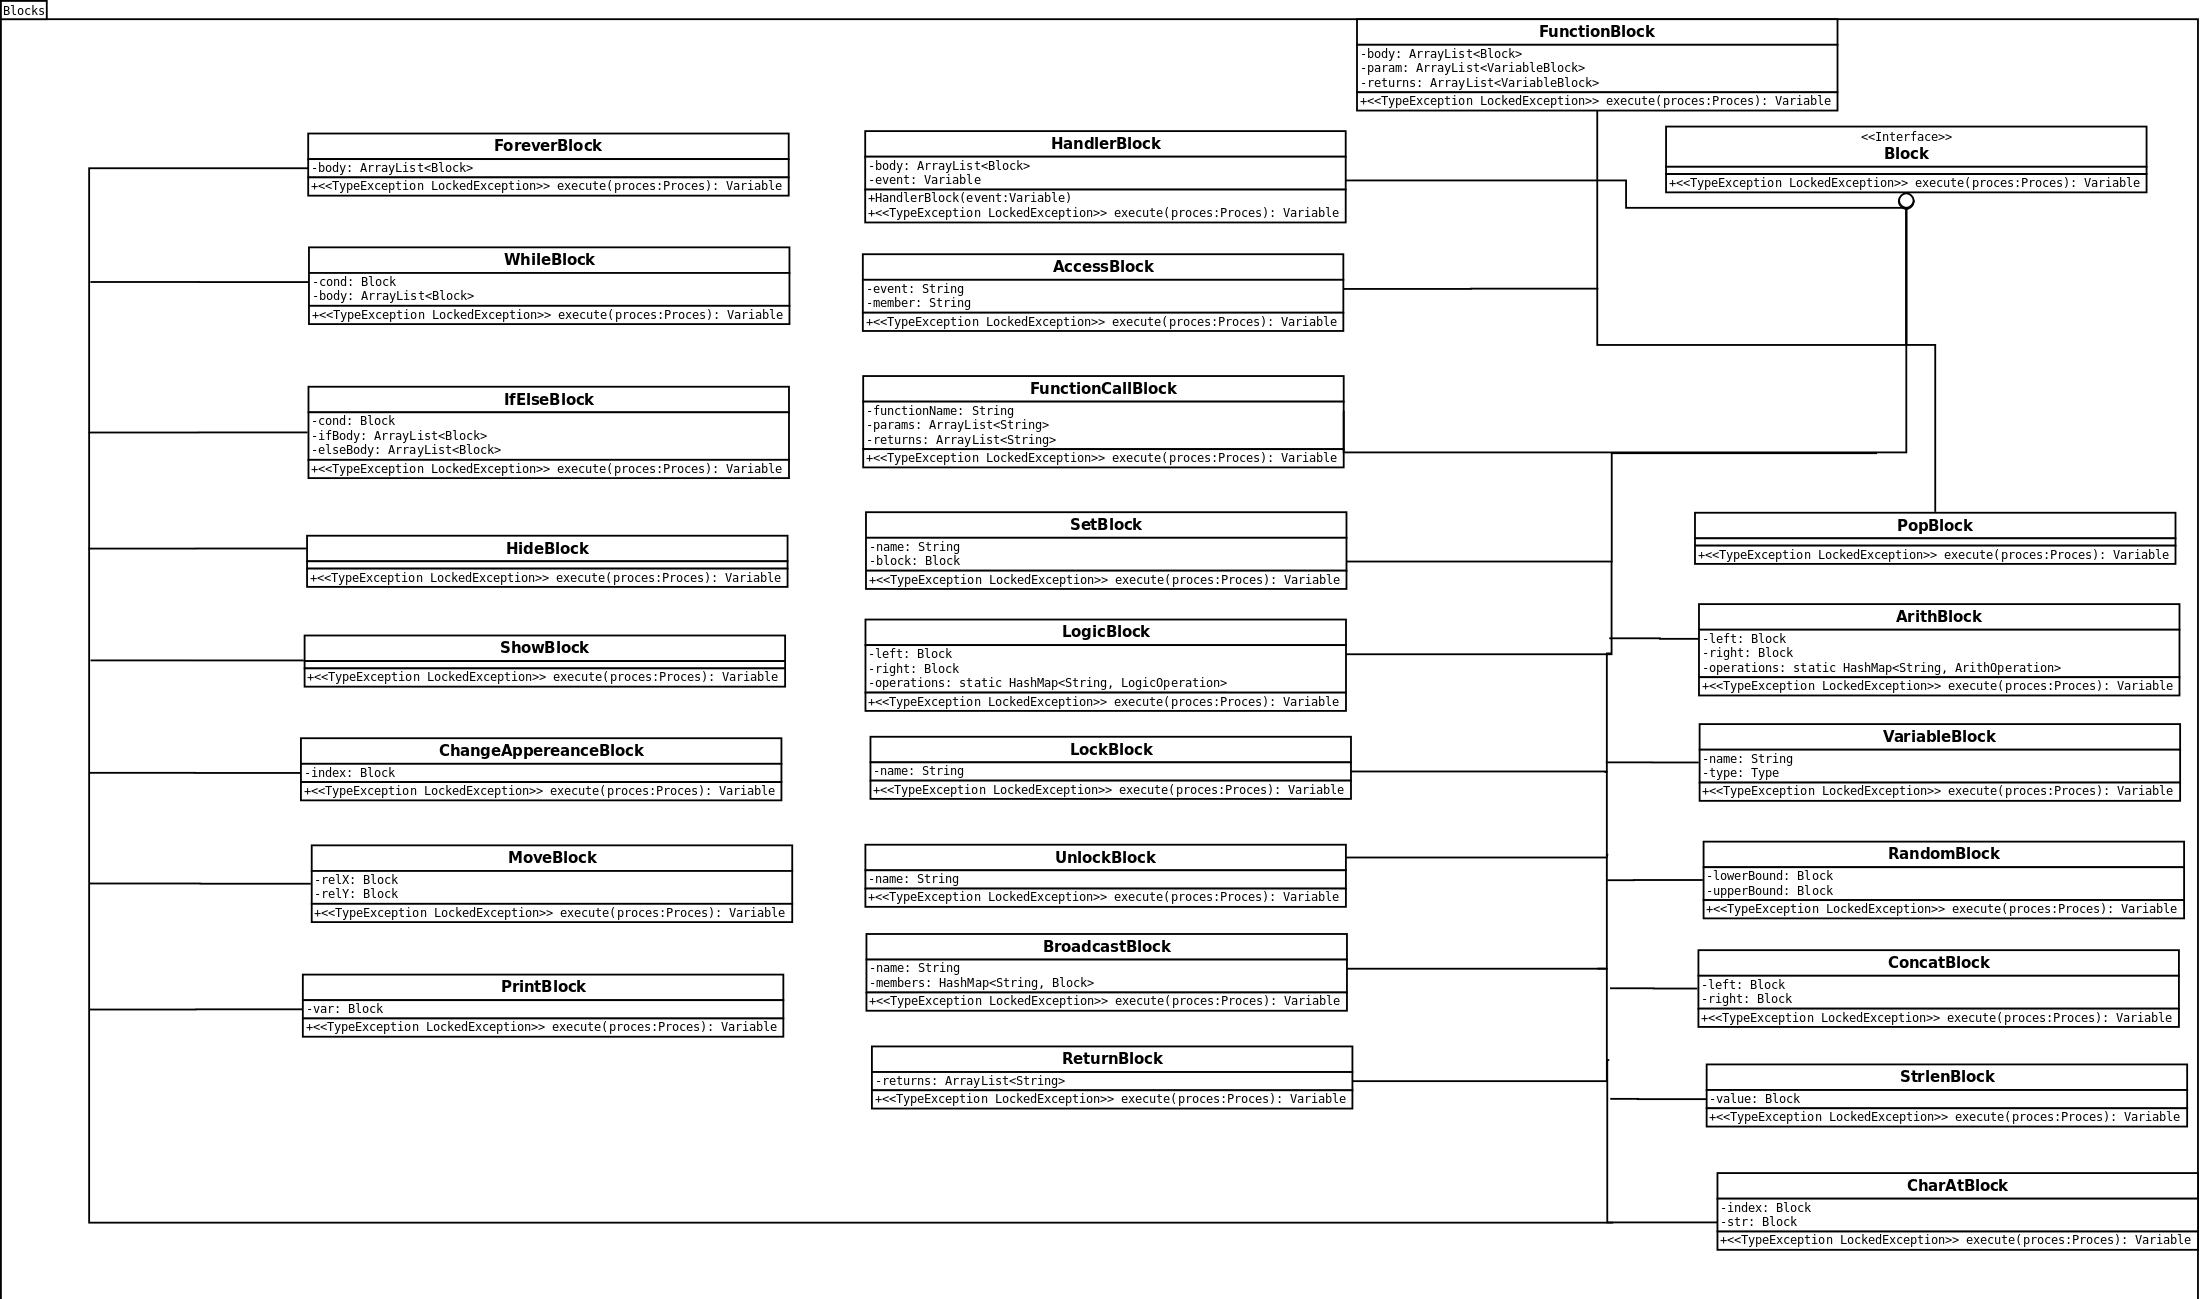
\includegraphics[scale=0.8]{./AnalyseClassenDiagram/block.png}
  \caption{Block Module.} \label{blockUML}
\end{sidewaysfigure}
\clearpage

\subsection{Collections}
De verantwoordelijkheden van deze module worden beschreven in Sectie \ref{CollectionsModule}.
\subsubsection{Classpool}
\label{ClasspoolClass}
Deze bevat alle Classes die aangemaakt zijn in het programma. Deze slaat hij op in een HashMap \cite{hashmap} waarbij een String (de naam) wordt gemapt op een Class. De naam van een Class moet dus uniek zijn.\\\\
\textBF{Keuze ADT's: }
De keuze van een HashMaps \cite{hashmap} zorgt ervoor dat het toevoegen van nieuwe items en het opzoeken van bestaande in O(1) tijd kan gebeuren.
\subsubsection{WiredInstance}
Een wiredInstance bevat een HashMap \cite{hashmap} waarbij een event wordt gemapt op een lijst van instances. We gebruiken hiervoor dus \texttt{java.util.Hashmap<Event, ArrayList<Instance>>} \cite{hashmap} \cite{arraylist}.  Dit stelt alle instances voor die verbonden zijn met \"{e}\"{e}n specifiek uitgaande event van \"{e}\"{e}n specieke instance.
\subsubsection{WireFrame}
\label{WireFrameClass}
Een WireFrame stelt de plaats voorwaarbij alles instanties met elkaar worden verbonden met wires.
Deze bevat een hashmap die Instances mapt op WiredInstances \cite{hashmap}.\\\\
\textBF{Keuze ADT's: }
Door gebruik te maken van deze structuur van Hashmap \cite{hashmap} en WiredInstance kunnen we snel toevoegen en opzoeken. Bij het toevoegen van een wire zal er voor de instance zijn wireFrame worden opgevraagt en voor het event dat verbonden wordt zal de instance waar de wire aankomt worden toegevoegd aan de bijhorende Arraylist \cite{arraylist}. Deze operatie duurt dan O(1) + O(1) + O(1).\\
Het opvragen van alle van instances die verbonden zijn met \'{e}\'{e}n event van \'{e}\'{e}n instance kan dus op dezelfde manier in O(1) + O(1).\\ Het is ons bekend dat het verwijderen van een wire op deze manier niet snel kan verlopen. Het verwijderen gebeurt echter niet op runtime. Daar is het zoeken van belang. We hebben dit in afweging genomen en hebben besloten te gaan voor het snel werken van de VM en dus gekozen voor snel opzoeken.
\subsubsection{EventPool}
\label{EventPoolClass}
Bevat alle Events die in het programma aangemaakt zijn. Deze bewaart hij in een HashMap \cite{hashmap} waarbij een String (het type) wordt gemapt op een Event. Het type van een Event moet dus uniek zijn (voor de hashmap).


\clearpage
 \begin{sidewaysfigure}
  \centering
   
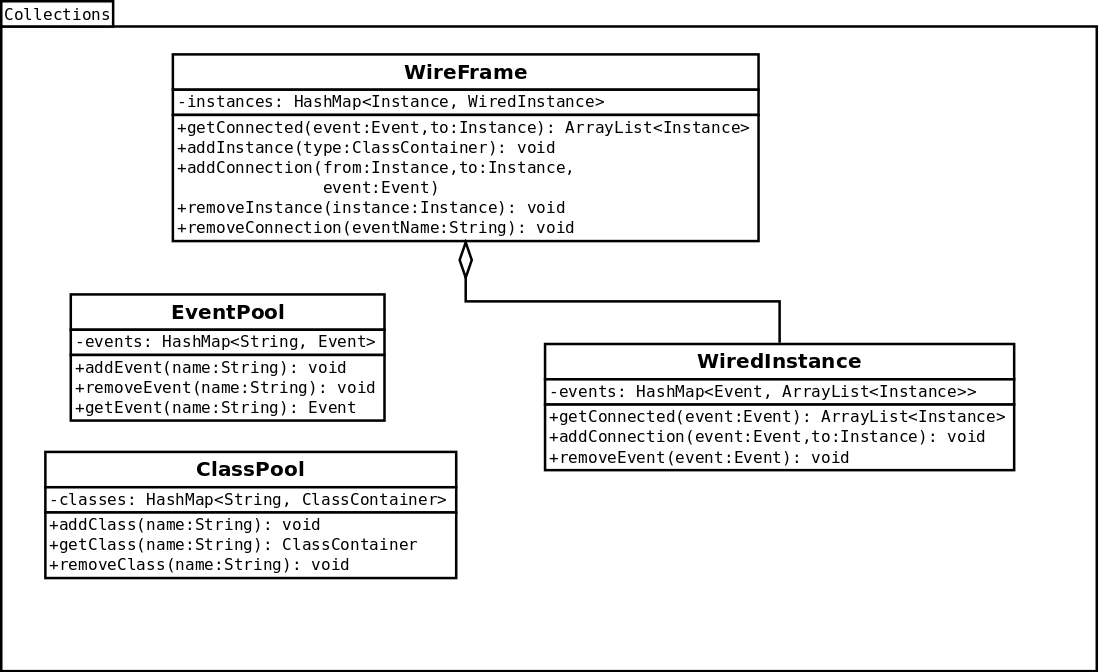
\includegraphics[scale=0.8]{./AnalyseClassenDiagram/collections.png}
  \caption{Collections Module.} \label{collectionsUML}
\end{sidewaysfigure}
\clearpage

\subsection{Core}
De verantwoordelijkheden van deze module worden beschreven in Sectie \ref{CoreModule}.
\subsubsection{Instance}
Deze klasse stelt een instantie van een Class voor. Deze bevat een HashMap \cite{hashmap} van variables deze zijn zijn member variables maar ook zijn positie. Een instance bevat ook zijn Class zodat men weet welke events en functies deze bevat. Een instance bevat ook een HashSet van zijn locked members. 
\subsubsection{EventDispatcher}
\label{eventdispatcher}
De EventDispatcher krijgt een eventInstance en een afzender van de virtual machine. De EventDispatcher kent alle wires en instances. Hij zal voor het gegeven eventInstance alle handlers van de ontvangers opvragen die voor dat event met de afzender zijn verbonden. Voor elke handler cree\"{e}rt hij een nieuw proces dat hij aan de virtual machine geeft.
\subsubsection{Proces}
\label{procesklass}
Het proces bevat een stack van Blocks. Initi\"{e}l bevat die stack enkel de handler die opgeroepen is. Het bevat de instantie waarvan het de handler uitvoert. Het bevat ook een Stack van functionFrames (van Hashmaps waarbij Strings worden gemapt op Variables (zie Sectie \ref{variable})(zie Sectie \ref{functionframe}).\\ Deze laatste stack stelt de stack van actieve functies voor. \\ Een proces bevat een run-functie die \'{e}\'{e}n primitieve stap zal uitvoeren. Deze functie kan een event teruggeven als deze gecree\"{e}rd werd in de primitieve stap. Als het geen event terug geeft is er geen event gecree\"{e}rt maar is het proces nog niet afgelopen. Als het wel een afgelopen (de stack van Blocks is leeg) zal het een ProcesFinishedException gooien. Hierdoor weet de virtualmachine dat het event niet terug op de queue moet worden gezet. Het proces bevat ook nog een klasse ReturnVariables.\\ De klasse bevat ook nog een boolean locked die aangeeft als het proces verantwoordelijk is voor het locken van een variabele. Hierop kunnen er wel nog nieuwe locks gebeuren binnen dat proces. Een voorbeeld van de werking van een proces is uitgewerkt in Sectie \ref{voorbeeldvm}.\\\\
\textBF{Keuze ADT's: }
\label{keuzeHashVar}
De Stack \cite{stack} van Blocks zorgt ervoor dat telkens de bovenste blokken geexecute kunnen worden. De functie wordt er dus telkens volledig bovenop gezet. Omdat we enkel bovenaan moeten toevoegen en uitvoeren gebeurt deze operatie in O(1). We gebruiken hiervoor \texttt{java.util.Stack<Block>} heb Voor informatie over het toevoegen van de blokken van een functie op deze stack verwijzen we naar de Class FunctieBlock.\\\\
Het gebruiken van een Stack \cite{stack} zorgt ervoor dat we weten in welk blok er gezocht moet worden naar de lokale variabele van de huidige functie. Hierdoor kan de totale operatie van zoeken in O(1). Als een variable niet gevonden wordt, zoekt men in de member variables van de instance.
\subsubsection{VirtualMachine}
\label{VMClass}
De virtual machine bevat een lijst (queue) van processen (zie Sectie \ref{procesklass})en de eventDispatcher. Hij doorloopt de lijst van processen door telkens de voorste eraf te halen. Hij zal elk proces \'{e}\'{e}n primitieve stap laten uitvoeren. Als het proces in die primitieve stap een event cree\"{e}rt zal de VM (virtual machine) dit event en zijn zender doorgeven aan de eventDispatcher. Zoals eerder vermeldt zal de eventDispatcher een hoeveelheid processen teruggeven (\texttt{ArrayList<Proces>} \cite{arraylist}). Deze worden achteraan de lijst toegevoegd. Als het huidige proces nog niet is afgerond wordt dit ook achteraan terug toegevoegd (na de eventuele nieuwe processen).\\\\
\textBF{Keuze ADT's: }
Voor de queue gebruiken we \texttt{java.util.LinkedList<Proces>} \cite{linkedlist} hierdoor kan het afnemen van het eerste element en toevoegen van een element aan de queue in O(1). Natuurlijk is de orde van belang in de queue wat hier FIFO is.\\
\subsubsection{FunctionFrame}
\label{functionframe}
Een functionFrame stelt het stackframe voor van een functie blok. Deze bevat een hashmap \cite{hashmap} waarbij
de lokale Variables van die functie gemapt worden op hun naam in die functie.\\\\
\textBF{Keuze ADT's: }
Een Hashmap waarbij Strings worden gemapt op variables. De keuze van een Hashmap zorgt ervoor dat het toevoegen van nieuwe variabelen en het opzoeken van bestaande in O(1) tijd kan gebeuren aangezien een functie een beperkt aantal lokale variabele bevat. Door het gebruik van een Hashmap is er ook geen compile stap nodig omdat we de variable dadelijk kunnen mappen op de content en geen indices van een array moeten worden berekent.\cite{hashmap}
\subsubsection{Event}
Een event bevat een String voor zijn type aan te duiden en een HashMap waarbij het de naam van een variable (String) mapt op een type van variabele. Deze klasse kan een EventInstance van dit event aanmaken \cite{hashmap}.
\subsubsection{Class}
Een Class bevat twee lijsten inputEvents en outputEvents die respecitievelijk alle inkomende en uitgaande events bevatten \cite{arraylist}. Een Hashmap van Strings gemapt op Types die zijn membervariabele voorstellen. De klasse bevat ook twee Hashmaps \cite{hashmap} functions en handlers die respecitievelijk  alle functies en alle handlers bevatten. Bij functions worden functies gemapt op hun naam en bij handlers worden gemapt op het event waarbij ze worden opgeroepen. Een Class is een factory voor zijn instances.

\clearpage
 \begin{sidewaysfigure}
  \centering
   
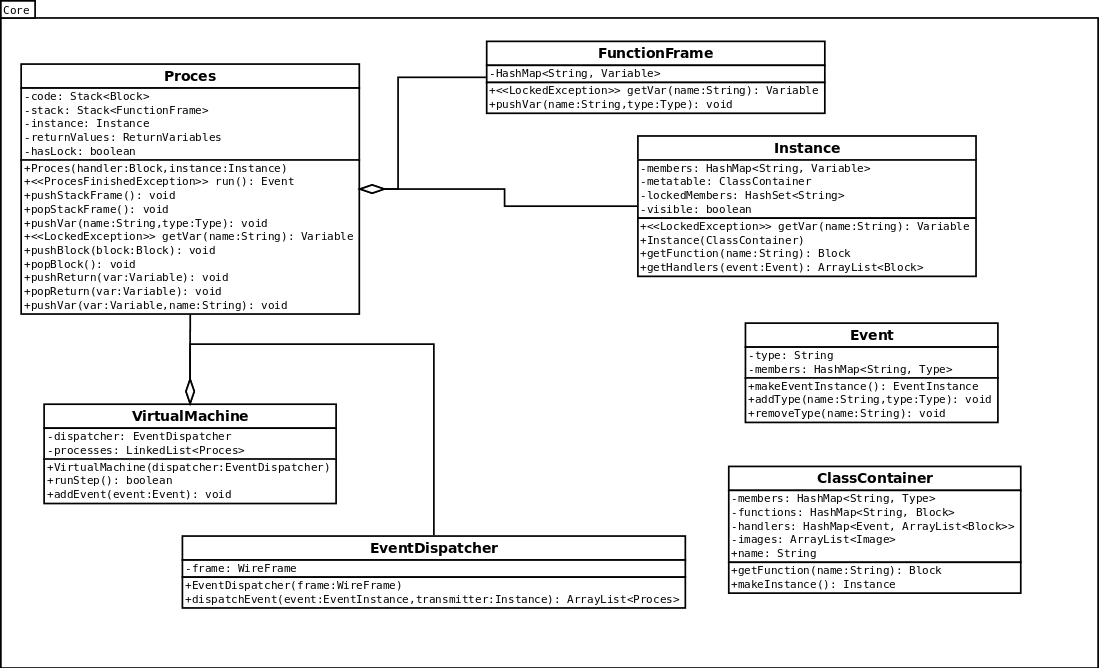
\includegraphics[scale=0.8]{./AnalyseClassenDiagram/core.png}
  \caption{Core Module.} \label{coreUML}
\end{sidewaysfigure}
\clearpage

\subsection{Model}
De verantwoordelijkheden van deze module worden beschreven in Sectie \ref{ModelModule}.
\subsubsection{Abstracte Klasse BlockModel}
\label{ModelBlock}
Deze abstracte klasse wordt als basis voor elk model van bruikbare blokken in de IDE. Deze bevat alle gemeenschappelijke attributen van alle modelen. Deze bestaan uit de positie van het view van die block in de klasse. Alsook een Boolean die aangeeft als de blok moet oplichten bij het debuggen.\\\\ Hieronder geven we enkele afgeleide blokken, een volledige beschrijving zo echter te verleiden voor dit verslag.
\subsubsection{ClassModel}
Deze klasse wordt gebruikt om een klasse in de IDE voor te stellen. Deze bevat de volgende attributen: Alle functieblokken, handlers, naam van de Klasse, outputEvents, member variabelen, images en floatingBlocks. Het gebruik van alle vorige attributen volgt logische uit de beschrijving van een Klasse. Behalve floatingBlocks deze wordt gebruikt voor het groeperen van alle blokken die de gebruiker op het veld van de Klasse heeft geplaats maar nog niet in een functie of handler heeft geplaatst.\\\\
\textBF{Keuze ADT's: }Voor het bijhouden van welk inputEvent wordt afgehandeld door welke handlers gebruiken we een HashMap die het EventModel mapt op een lijst van handlers. Hiervoor gebruiken we \\ \texttt{java.util.Hashmap<EventModel,java.util.ArrayList<HandlerModel>>}. \\ Voor de het bewaren van de member variabele en hun type gebruiken we een Hashmap die de naam van de variabele mapt op een Type \ref{Type}. Hiervoor gebruiken we \texttt{java.util.Hashmap<String, Type>}.
\subsubsection{WhileModel}
Dit is een voorbeeld uitwerking van een BlockModel voor een programmeerblokje. De klasse van een  programmeerblok model die andere blokken kan bevatten heeft voor alle blokken van die klasse een statische lijst van alle BlockModel's die de blok mag bevatten. Aangezien een While-blok twee input velden heeft, scheiden we deze hier door een conditieModel die hier verder wordt uitgewerkt en een lijst van blokken die geaccepteerd zijn in de body.\\\\
\textBF{Keuze ADT's: }
Voor het bijhouden van welke blokken een blok mag bevatten gebruiken we een \texttt{java.util.HashSet<Class>}. Hiermee kan dan worden nagegaan als een blok in een andere kan worden geplaatst. We kiezen voor een HashSet zodat het controlleren een constante tijd kan gebeuren.
\subsubsection{WireFrameModel}
Door dat de compiler de juiste compile functie zoekt op het type, is het WireFrame ook een BlockModel. Deze klasse bevat alle instanties die in het frame staan als ook de wires die ze verbinden. Beide worden bijgehouden in een lijst.
\subsubsection{WireModel}
Dit is een blockModel om een wire voor te stellen. Deze bevat een InstanceModel waarvan het vertrekt en een waar het aankomt. Ook weet de wire welk event het verstuurd.
\subsubsection{InstanceModel}
Dit is een model voor een instance in het WireFrame. Een Instance hoort bij een Klasse. Daarom zal hij de Klasse waarvan hij een instantie is observeren voor veranderingen.

\clearpage
 \begin{sidewaysfigure}
  \centering
   
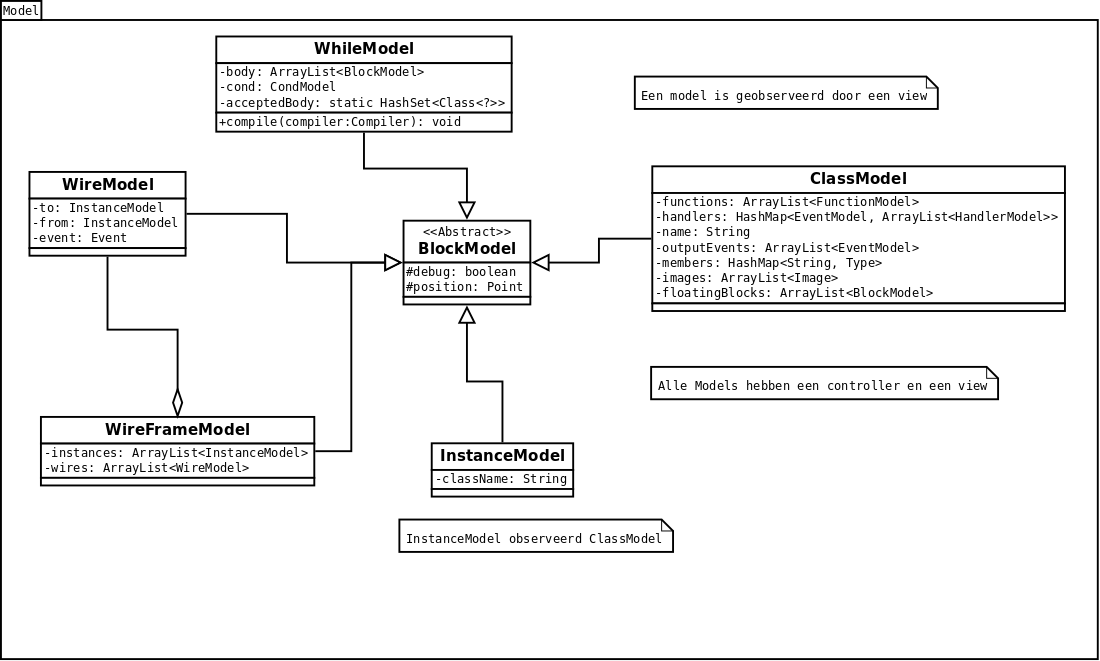
\includegraphics[scale=0.8]{./AnalyseClassenDiagram/model.png}
  \caption{Model Module.} \label{modelUML}
\end{sidewaysfigure}
\clearpage

\subsection{RunTime}
De verantwoordelijkheden van deze module worden beschreven in Sectie \ref{RuntimeModule}.
\subsubsection{Abstracte Klasse Runtime}
Deze klasse wordt gebruikt voor het uitvoeren van het gecree\"{e}rde programma. Alle Klassen en hun blokken zullen eerste door een Compiler die deze klasse bevat gecompileerd worden. Na het succesvol compileren zal de Runtime verantwoordelijk zijn voor het starten van de virtual machine, het stoppen ervan en het doorgeven van inputEvents veroorzaakt door de gebruiker aan deze virtual machine.
\subsubsection{InterpeterRuntime}
\label{runtimeClass}
Dit is de runtime die ge\"{i}mplementeerd zal worden voor dit project. Deze bevat een virtual machine die beschreven wordt in Sectie \ref{VMClass}. De compiler die wordt gebruikt in dit project wordt beschreven in Sectie \ref{IntCompClass}. Deze compiler vult de attributen Classpool, EventPool en WireFrame in deze worden respectievelijk beschreven in Sectie \ref{ClasspoolClass}, Sectie \ref{EventPoolClass} en Sectie \ref{WireFrameClass}.
\subsubsection{Interface Compiler}
We voorzien een Interface voor de compiler zodat er makkelijk een andere compiler kan worden ge\"{i}mplementeerd. Deze bevat een functie voor het compileren van een Runtime.
\subsubsection{InterpeterCompiler}
\label{IntCompClass}
Deze klasse bevat de compiler die ge\"{i}mplementeerd zal worden voor dit project. De bevat functies voor het compileren van een model. Een gedetailleerd beschrijving is te vinden in Sectie \ref{Compileer}.

\clearpage
 \begin{sidewaysfigure}
  \centering
   
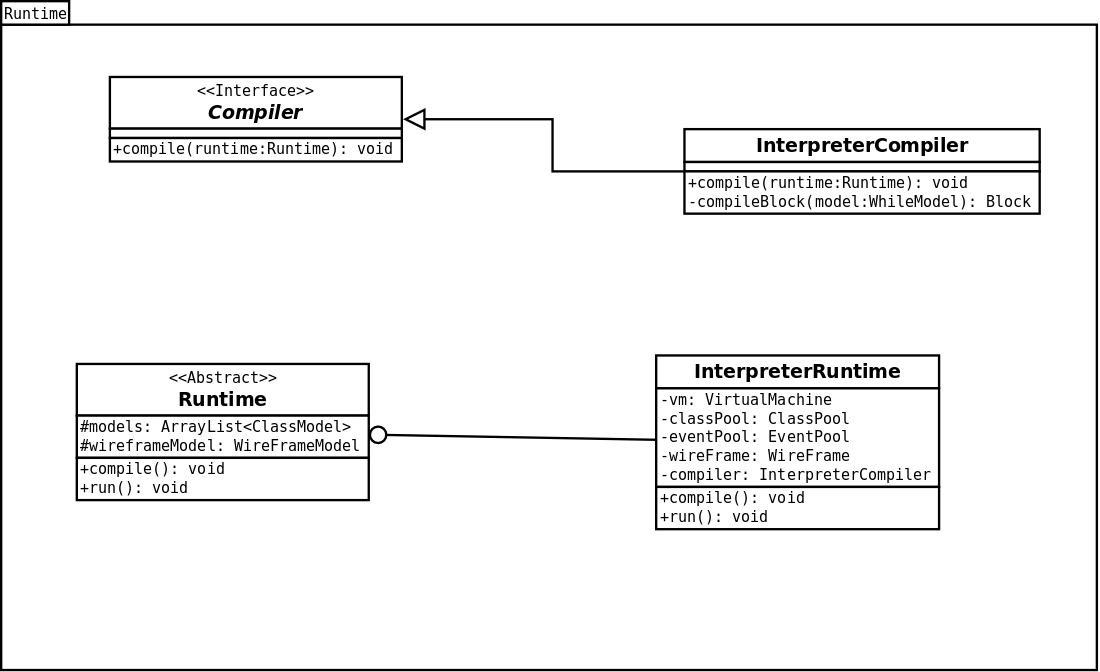
\includegraphics[scale=0.8]{./AnalyseClassenDiagram/runtime.png}
  \caption{Runtime Module.} \label{runtimeUML}
\end{sidewaysfigure}
\clearpage

\subsection{File}
\subsubsection{LanguageModule}
De language class zorgt voor het multilanguage maken van de IDE. Dit gebeurt door een \texttt{ResourceBundle} zoals uitgelegd in Sectie \ref{Multilanguage}

\subsubsection{DataParser}
Een interface klasse die de IDE gebruikt om data te schrijven naar een file. Deze data zal bestaan uit de informatie zijn die nodig is voor projecten die bestaan uit Events, Instanties, Klassen en gerelateerde data.

\subsubsection{XMLParser}
Dit is een implementerende klasse van een DataParser. Deze klasse wordt gebruikt om XML data  te lezen en te schrijven naar een bestand. De XML parser is een information expert met betrekking tot XML data, hij bevat functies waarmee de Modellen van een Klasse, Instantie, enz. geschreven en gelezen kunnen worden. De XML data zelf wordt geparsed door een \texttt{DOMParser} van de Java Standard Library.

\clearpage
 \begin{sidewaysfigure}
  \centering
   
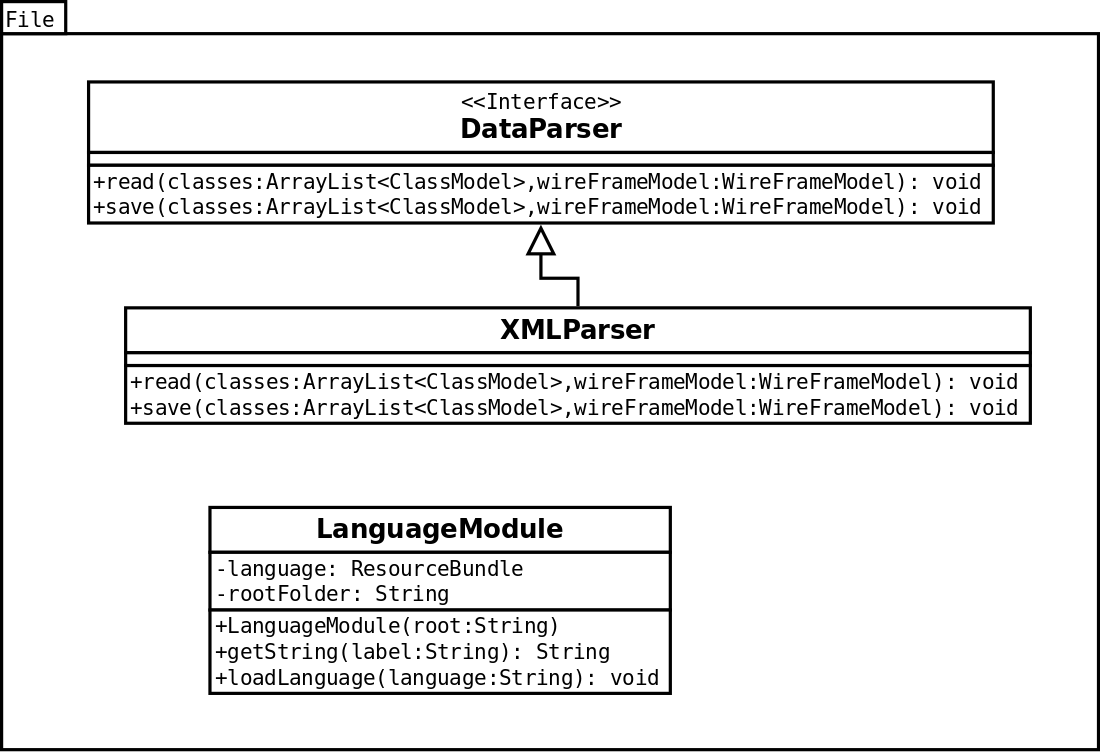
\includegraphics[scale=0.8]{./AnalyseClassenDiagram/file.png}
  \caption{File Module.} \label{file}
\end{sidewaysfigure}
\clearpage


\subsection{GUI}
In dit verslag is enkel de Main klasse uitgewerkt. Dit is de klasse die het JFrame zal bevatten alsook andere noodzakelijke data. Onder andere bevat deze klasse een LanguageModule, een DataParser, een Runtime en Modellen van aangemaakte Klassen/WireFrame

 \begin{figure}[h]
  \centering
   
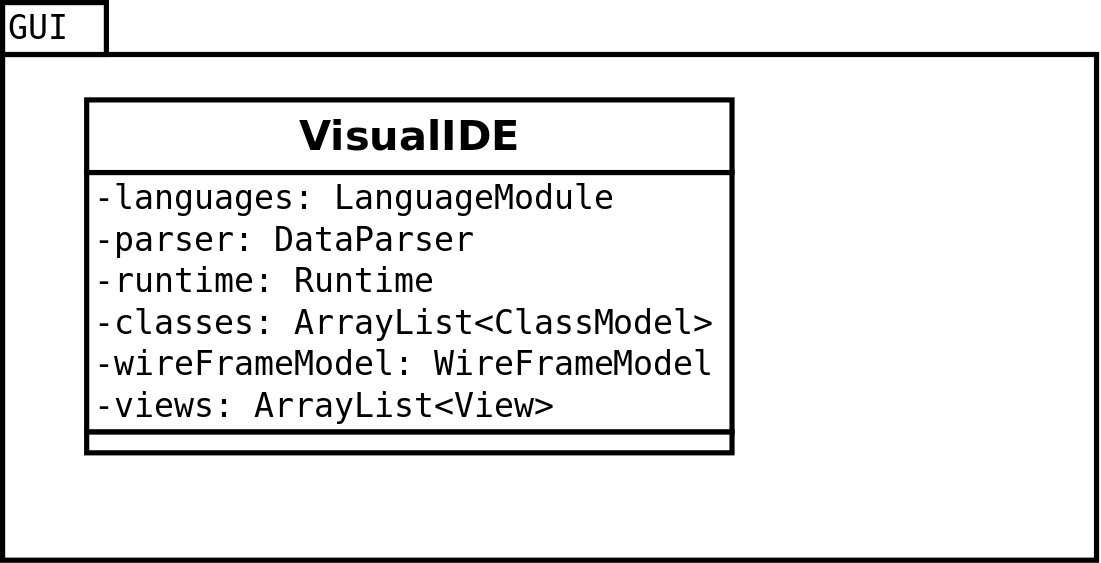
\includegraphics[scale=0.4]{./AnalyseClassenDiagram/gui.png}
  \caption{GUI Module.} \label{gui}
\end{figure}
\clearpage


 
\end{document}
\documentclass[]{article}

\begin{document}

\section{Opslaan en Inladen}
Deze sectie bespreekt hoe een bestand wordt opgeslaan en hoe problemen bij het inladen van een semantisch incorrect programma worden afgehandeld. Daarna wordt ook besproken hoe ondersteuning voor meerdere talen mogelijk werd gemaakt in de appplicatie.
\subsection{Keuze XML}
\label{XML}
Voor het opslaan van een programma moest een leesbaar formaat worden gekozen. Eerder in dit verslag werd al aangehaald dat een programma kan beschouwd worden als een boom structuur. De combinatie van deze twee aandachtspunten en het bestaan van betrouwbare verwerkings bibliotheken voor XML hebben ervoor gezorgd dat er gekozen werd voor XML.\\\\
In het analyseVerslag werd er gesteld dat data wordt opgeslagen naar meerdere files. Dit is echter een vervelende implementatie omdat de IDE dan meerdere files aanmaakt die aanpasbaar moeten zijn door de gebruiker. Voor de gebruiker is het simpelder indien er slechts \`e\`en XML file was om aan te passen. De beschrijving van de XML voor alle ge\"{i}mplementeerde blokken en XML DTD is achteraan beschreven in bijlage \ref{bijlagexml}.\\\\
Het volgende deel van deze sectie beschrijft de eigenlijke implementatie van het opslaan en inlezen van een programma. Als ook het afhandelen van een semantisch incorrect programma bij inladen.
\subsection{Opslaan en inladen van een programma}
\label{saveLoad}
Deze sectie beschrijft kort hoe een programma wordt opgeslaan en hoe het wordt ingeladen. Voor het inladen worden ook complexere zaken zoals het inladen van variabelen en functies besproken. Alsook de gevolgen van het inladen van een semantisch foutief programma.
\subsubsection{Opslaan}
Het opslaan van een progamma gebeurt in XML. Dit zal gebeuren zoals beschreven in Bijlage \ref{bijlagexml}. \\\\
Voor het opslaan wordt gebruik gemaakt van de boomstructuur gecre\"{e}rd door de \textbf{modellen} (Sectie~\ref{Modellen}) deze zijn centraal verzameld in de ModelCollection (Sectie~ \ref{ModelCollection}). Er is dus enkel nood aan een module die deze boom structuur afloopt en opslaat naar een bestand. Echter hebben we ervoor gekozen om het opslaan van een model los te koppelen van hun klasse. Dit om de klasse niet te vervuilen en de mogelijkheid te hebben om gemakkelijk een ander bestandsformaat te kiezen voor het opslaan van een programma. Er werd een Interface DataSaver ge\"{e}implementeerd die deze uitbreidbaarheid verzekerd.\\\\
Hierdoor duikt er in Java het probleem op waarbij er niet automatisch de functie wordt genomen met de meest specifieke klasse van een instantie. Om dit op te lossen werd er ook hier gebruik gemaakt van het Visitor patroon zoals beschreven in Sectie~\ref{visitorpatroon}\\\\
Voor het opslaan van \textbf{kostuums} van een klasse hebben we gekozen om de ingeladen afbeeldigen te kopi\"{e}ren naar de folder waar de gebruiker het programma wenst op te slaan. Elke afbeelding wordt hernoemt naar een combinatie van de gekozen kostuums naam en de klasse waarbij deze behoort. De paden van de afbeeldingen worden relatief opgeslaan t.o.v de gekozen folder. 
\subsubsection{Inladen}
Voor het inladen van het programma wordt ge\"{e}ist dat de XML correct gedefinieerd is. Bijlage \ref{bijlagexml} beschrijft deze definitie. De volgende paragrafen beschrijven het gedrag van de applicatie bij gebruik van incorrecte semantiek in verschillende delen van het bestand.
\paragraph{Events}
Als eerste worden de Events ingeladen. Aangezien deze overal in het programma kunnen gebruikt worden. Een Event moet uniek zijn. Bij het inlezen van een duplicaat Event zal dit Event worden overgeslaan. De members van een Event moeten uniek zijn. Bij het inlezen van een duplicate member zal deze member worden overgeslaan.\\\\
Bij het inlezen van blokken die gebruik maken van Event zal het bestaan van het Event gecontrolleerd worden. 
\paragraph{Variabelen}
Het programma wordt per klasse ingeladen. Klasse naam moet uniek zijn. Duplicate namen worden overgeslaan. Voor een klasse worden eerst de membervariablen ingeladen ook deze moeten uniek zijn. Membervariabelen worden gestokeerd in een lijst. Bij het inlezen van handler of functie zal deze lijst worden aangevuld als er een definitie van een lokale variable wordt ingelezen.\\\\
Bij het inlezen van een referentie naar een variable wordt nagekeken als deze variablen gedefinieerd is. Zoja, dan wordt er een referentie naar deze variable gecree\"{e}rd. Anders zal de referentie niet worden ingeladen. Maar het programma wordt wel verder ingeladen. Voor elke functie of handler wordt er vertrokken vanuit de lijst met member variabelen.
\paragraph{Functies}
Functies moeten een unieke naam hebben. Bij een duplicate functie wordt deze overgeslaan.
\paragraph{Functie aanroepen}
Bij het tegenkomen van een functie oproep wordt deze ingeladen en ingevuld met de gewenste parameters en return. Echter worden alle functie oproepen apart opgeslaan zodat deze later gekoppeld kunnen worden aan hun gewenste functie. Als na het inlezen van alle functies, de functie waarnaar de functie oproep refereert niet gevonden is, zal het programma niet worden ingeladen.
\paragraph{Handlers}
Als bij het inladen van een Handler een onbekend Event wordt gegeven zal deze handler geen Event worden toegekend. De handler en zijn body worden wel ingeladen.
\paragraph{Kostuums}
Bij ongeldig pad naar een afbeelding of het beschreven bestand is geen afbeelding zal de er geen afbeelding worden getoond in het programma maar zal het inladen gewoon verder gaan. 
\paragraph{Instanties}
De naam van een instantie moet uniek zijn. Bij het inladen van een duplicate instantie zal deze worden overgeslaan.
\paragraph{Wires}
Duplicate wires worden overgeslaan. Bij het inladen van een wire tussen onbekende instanties of met een onbekend Event. Zorgt ervoor dat vanaf dat punt geen instanties of wires worden ingeladen.
\subsection{Multilanguage IDE}
\label{Multilanguage}
De visuele programmeer IDE moet multilanguage zijn. De gebruiker moet kunnen wisselen tussen verschillende talen. Aangezien we Java gebruiken zijn we gaan kijken naar standaard klassen om multilanguage applicaties te maken. De oplossing is de ResourceBundle Class die Java aanbiedt \cite{javabundle}.

Een ResourceBundle laad automatisch de nodige file gegeven een bepaalde filenaam (en eventueel een locale). Vervolgens kan via een getString("label") de tekst in de gevraagde taal opgevraagd worden. Een locale beschrijft een bepaalde taal, zo kan er een UK engels, en een US engels gemaakt worden \cite{javalocale}. Hieronder staat beschreven hoe de files voor verschillende talen genoemd moeten worden. De inhoud van deze files volgt een simpel formaat nl, key = tekst \cite{jenkov}.\\
Voorbeeldcode: \cite{jenkov}
\lstset{language=Java}
\begin{lstlisting}
public class Main {
	public static void main(String[] args) {
		// De constructor heeft 2 parameters:
		//	een taal en een land
		Locale locale = new Locale("en", "UK"); 
		// language.properties is een file
		ResourceBundle language = ResourceBundle.getBundle("language", locale);
		System.out.println(language.getString("label"));
	}
}
\end{lstlisting}
De verschillende files:
\lstset{language=XML}
\begin{lstlisting}
language.properties
language_en.properties
\end{lstlisting}
Een mogelijke inhoud van \texttt{language.properties}: 
\lstset{language=XML}
\begin{lstlisting}
label1 = een bepaalde tekst
label2 = een andere tekst
\end{lstlisting}
Een mogelijke inhoud van \texttt{language\_en.properties}: 
\lstset{language=XML}
\begin{lstlisting}
label1 = a certain text
label2 = another text
\end{lstlisting}



\subsection{Omzetting van Modellen naar Views}
Bij het gebruik van GUI zal elk view eerst bij reset de bestaande modellen opvragen en hiervoor views cree\"{e}ren. Voor het inladen van een klasse zullen de blokken ingeladen worden en gekoppeld worden aan views. Dit is mogelijk aangezien een View kan werken door views aan elkaar toe te voegen maar ook door enkel modellen te koppelen.\\\\ Het aanmaken van de Views wordt gedaan door de LoadClassViewFromModel klasse. Deze zal de blokken van een ClassModel koppelen aan hun views en op het IDEPanel plaatsen. Hier werdt er geen gebruik gemaakt van het Visitor patroon zodat een model niet vervuild wordt met de functionaliteit van view creatie.


\end{document}

\documentclass[]{article}

\begin{document}

\section{Mockups}
\label{Mockups}
\subsection{Menubalk}
In de menubalk van de applicatie vindt de gebruiker onder Bestand de mogelijkheid terug om een programma op te slaan, in te laden of om een nieuw programma te maken. Bij instellingen kan hij de console aan en uitzetten en de taal van de applicatie veranderen.\\In het midden van de menubalk vinden we een start knop waarmee de uitvoering van het programma wordt gestart mits het correct geconstrueerd is. Hiernaast bevindt zich ook de knop om de uitvoering te stoppen.\\ Aan de rechterzijde bevindt zich een switch bestaande uit drie knoppen: Klasse, Kabels en Events. Deze stellen de verschillende delen van de IDE voor die gebruikt worden om een programma te cree\"{e}ren. De beschrijving van deze delen op hoog niveau staat in Sectie \ref{interpretatie}.
\subsection{Klasse creatie}

Bij het selecteren van Klasse in de switch zal aan de gebruiker het klasse creatie view getoond worden. De mockup van dit view is te zien op figuur \ref{creatieklassemockup}. Hierin vindt hij onder de menubalk een balk waarin de reeds gecree\"{e}rde klasse zich als tabbladen bevindt. Op het einde van deze balk bevindt er zich een plus toets waarmee een nieuwe klasse kan worden toegevoegd.\\\\Aan de linkerzijde vindt de gebruiker alle categorie\"{e}n van de programmeerblokken. Bij het selecteren van een categorie zullen alle blokken die tot die categorie behoren verschijnen onder de categorie\"{e}n. Bij het aanklikken van een blok zal deze op het creatie veld verschijnen.\\\\ De kleuren en vorm van blokken, types en events moet nog aangepast worden op het eenvoudige gebruik van de applicatie en het proffesionele uitzicht ervan. Onderstaande mockups dienen voor het aantonen van de werking van de applicatie.\\ Het inelkaar klikken van blokken zal op een intu\"{i}tieve manier moeten duidelijk worden gemaakt. Als een blok de andere niet accepteerd zal deze er boven op blijven zweven maar zal het voor de gebruiker duidelijk zijn dat de blokken niet verbonden zijn.\\\\ Het verbinden van input events met de handler die de gebruiker wenst gebeurt met pijlen. Hierbij zal een pijl enkel kunnen verbonden worden als de handler ook het juiste event als input parameter heeft.\\ Het definieren van een functie gebeurt doormiddel van een functieblok. Deze kan de gebruiker een naam geven. Voor het toevoegen van een parameter moet de gebruiker op plus tekenen duwen en een variable en een type invullen. Het oproepen van een functie kan met een functiecallblok. Deze bestaat uit een blokje waaraan een pijl zit met een andere blok waarin de gebruiker een functie kan selecteren uit een lijst van functies uit die klasse. Onderaan dit blok kan een blokje staan waarin de return waarde van de functie kan worden opgevangen.\\\\ Aan de rechterzijde van de klasse creatie bevinden zich alle uitlijken van die tot een klasse behoren. Zo kan een klasse lamp bijvoorbeeld twee uitlijken bezitten namelijk een uit en aan afbeelding. Deze kan dan worden veranderd door een verander van uiterlijk blok.\\Hieronder bevinden zich de member variable van de klasse. Deze kan de gebruiker aanmaken door op het plus teken te drukken en een variabele van het gewenste type aan te maken met een unieke naam. Hiervan kunnen dan blokken op het creatie veld worden geplaats om te gebruiken in functies of handlers. Tenslotte vind de gebruiker hieronder alle events die hij reeds gedefineerd heeft in de event sectie van de IDE. 


 \begin{sidewaysfigure}
  \centering
   
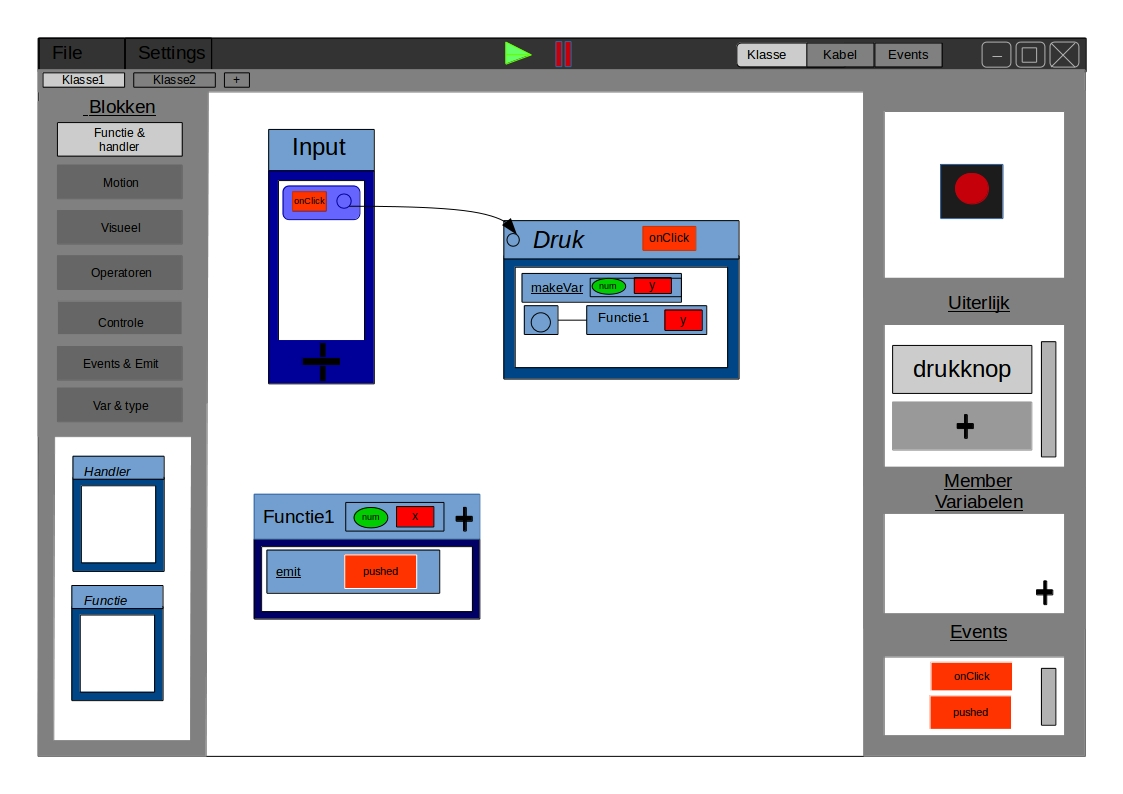
\includegraphics[scale=0.5]{../mockups/MockupCreatie.jpg}
  \caption{Mockup creatie klasse.}
  \label{creatieklassemockup}
\end{sidewaysfigure}
\clearpage
\subsection{Creatie instanties en kabels}
In dit view kan de gebruiker het hogere niveau van de werking van zijn programma definieren. De mockup van dit view is te zien op figuur \ref{wireframemockup}. Dit doet hij door instanties aan te maken van zijn eerder gedefineerde klassen. Hiervan heeft hij dan de keuze om de uitgaande events en inkomende event met elkaar te verbinden met behulp van pijlen. Hiermee kan hij beslissen aan welke instantie hij een event doorgeeft.\\ Bij een programma met veel kabels kan dit al snel voor een hele cluster zorgen. Daarom wordt er een filter voorzien waarmee de gebruiker kan bepalen van welke klasses hij geen kabels toont of welke event kabels hij niet toont.
\clearpage
 \begin{sidewaysfigure}
  \centering
   
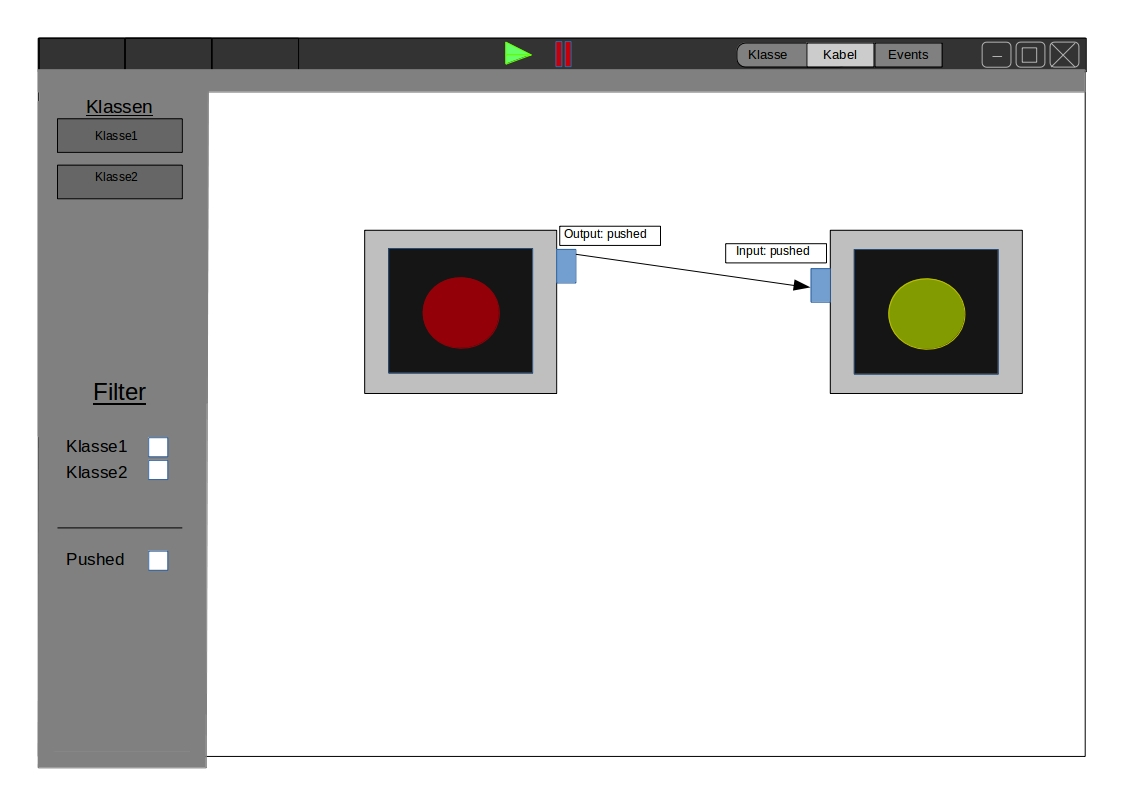
\includegraphics[scale=0.5]{../mockups/MockupWire.jpg}
  \caption{Mockup WireFrame.}
  \label{wireframemockup}
\end{sidewaysfigure}
\clearpage
\subsection{Event creatie}
In dit view kan de gebruiker een nieuw event defini\"{e}ren of een eerder gedefineerd event aanpassen. De mockup van dit view is te zien op figuur \ref{eventcreatiemockup}. Aan linkerkant van het venster bevindt er zich een overzicht van alle reeds gedefineerde events. Om een member aan het event toe te voegen gebruikt hij de plus knop en dan kan hij een member toevoegen van een gewenst type met een unieke naam. Een eerder toegevoegde member kan makkelijk verwijderd worden.
\clearpage
 \begin{sidewaysfigure}
  \centering
   
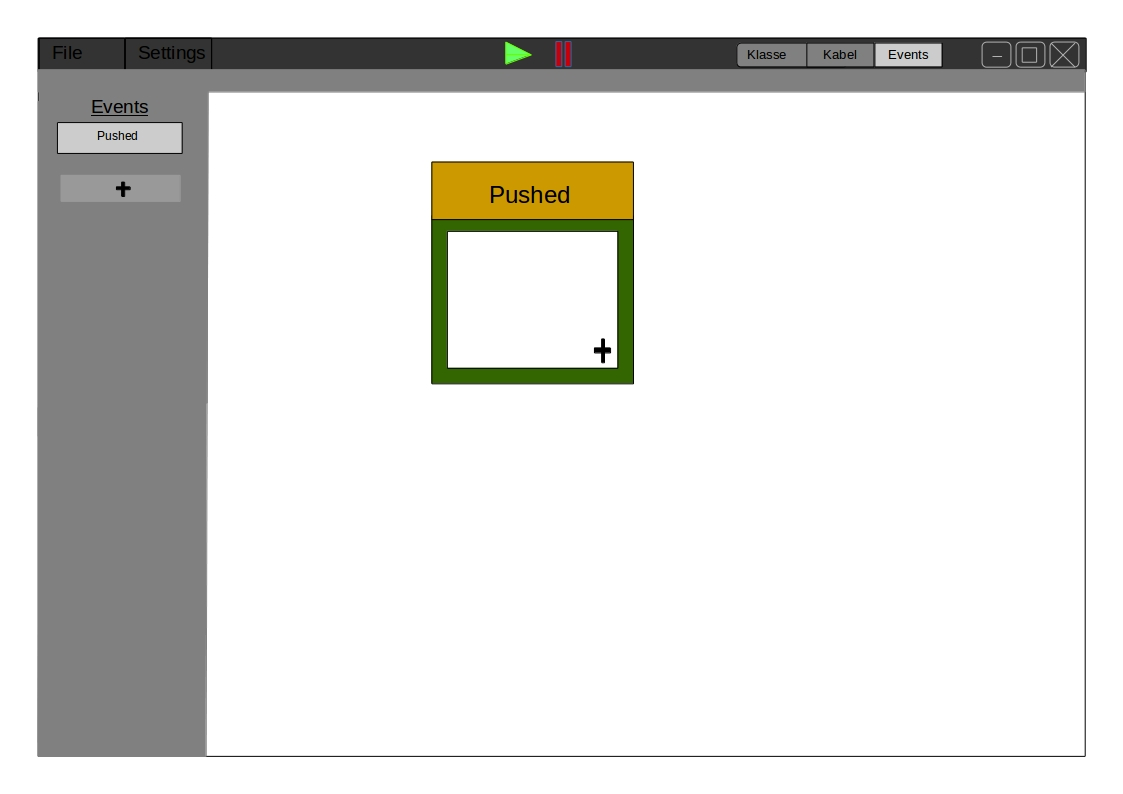
\includegraphics[scale=0.5]{../mockups/MockupsEvents.jpg}
  \caption{Mockup creatie event.}
  \label{eventcreatiemockup}
\end{sidewaysfigure}
\clearpage

\end{document}
\documentclass[]{article}

\begin{document}

\section{Taakverdeling en Planning}
\label{Taakverdeling}

\subsection{Planning}
We werken iteratief aan het software project. Er wordt gezorgd dat het eindverslag wekelijks bijgewerkt wordt. Voor de verschillende modules wordt eerst de kern ge\"{i}mplementeerd zodanig dat er een basis versie van het project bestaat. Deze versie word in verdere weken uitgewerkt tot een finale versie. In deze lijst staan telkens de belangrijke elementen die die week ge\"{i}mplementeerd worden.
\begin{itemize}
\item Week 1: Exceptions en Variables module maken. Aanmaak van enkele blokken uit de Blocks Module om te kunnen testen. Beginnen aan het aanmaken van de Core module
\item Week 2: Aanmaken van de Core module zodanig dat de Virtual machine operationeel is. Aanmaak XML inlezing zodat programma's al gemaakt kunnen worden in XML formaat. Hierdoor kan de Core module al volledig getest worden.
\item Week 3: Aanmaken Collections en Runtime module. Hierdoor ligt een basis voor de GUI klaar 
\item Week 4: Aanmaken van een eerste GUI prototype (en de multilanguage klasse) en de blok modellen.
\item 30 April 2015: Tussentijdse rapportering met opdrachtgevers.
\item Week 5: Verdere implementatie van alle blokken.
\item Week 6: Professioneel look geven aan de GUI.
\item Week 7: GUI verder afwerken en de blokken en hun modellen volledig afwerken.
\item Week 8: Extra tijd om extra's te implementeren of eventuele achterstand in te halen.
\item Week 9: Extra tijd om extra's te implementeren of eventuele achterstand in te halen.
\item 4 Juni 2015: Inleveren eindverslag en project.
\item 9 Juni 2015: Eindpresentatie finale software project.
\end{itemize}

\subsection{Taakverdeling}
Hierin staat beschreven wie welke onderdelen van een bepaalde module implementeerd. 
\begin{itemize}
\item Exceptions module: Matthijs implementeerd alle exceptions
\item Variables module: Axel implementeerd deze module volledig. 
\item File module: Language klasse wordt gemaakt door Axel
\item File module: Aangezien de dataparser klasse zeer groot is (zo'n 40 functies) zal ieder van ons de helft van deze functies implementeren. Deze functies zijn gericht op implementatie (een functie kan een while loop inladen of opslaan). Hierdoor is er nog geen exacte opsplitsen voor wie welke functie implementeert.
\item Core module: Axel implementeerd de Instance, Class, Proces en FunctionFrame. Matthijs maakt de Virtual Machine, Event en de Event Dispatcher.
\item Collections module: ClassPool en EventPool klassen worden gemaakt door Axel. De WireInstance en het WireFrame worden gemaakt door Matthijs. 
\item Runtime module: Matthijs maakt de Runtime. Aangezien de compiler klasse zeer groot is (zo'n 40 functies) zal ieder van ons de helft van deze functies implementeren. Deze functies zijn gericht op implementatie (een functie kan een while loop compiler bv). Hierdoor is er nog geen exacte opsplitsen voor wie welke functie implementeert.
\item Block module: Aangezien deze module zeer groot is (zo'n 40 klassen) zal ieder van ons de helft van deze klassen implementeren. Deze klassen zijn gericht op implementatie (een klasse kan een while loop voorstellen). Hierdoor is er nog geen exacte opsplitsen voor wie welke klasse implementeert.
\item Model module: Aangezien deze module zeer groot is (zo'n 40 klassen) zal ieder van ons de helft van deze klassen implementeren. Deze klassen zijn gericht op implementatie (een klasse kan een while loop voorstellen). Hierdoor is er nog geen exacte opsplitsen voor wie welke klasse implementeert.
\item Drag en drop: Dit wordt eerst samen bekeken. Zodat we goed weten hoe dit ge\"{i}mplementeerd moet worden.
\item WireFrame view: Matthijs implementeerd de WireFrame view (en andere benodigde views hierbij).
 
\item Event view + menu balk: Axel implementeerd de event view (en andere benodigde views hierbij) alsook de menu balk.

\item Programmeer view: Dit gaat opnieuw een grote hoeveelheid klassen zijn (voor de verschillende views van de verschillende blokken). Aangezien dit veel werk is, worden deze klassen opgesplitst. 
\end{itemize}

\end{document}
\documentclass[]{article}


\begin{document}

\bibliography{./Bibliografie/bibliografie}{}
\bibliographystyle{ieeetr}

\end{document}
\documentclass[]{article}

\begin{document}

\section{Log}
\begin{itemize}
\item 7 januari 2015: Keuze top 3 onderwerpen en motivatie.
\item 20 januari 2015: Voorbereiding mockups voor opdrachtgever.
\item 26 januari 2015: Meeting met opdrachtgever.
\item 27 januari 2015: Mockups en verslag van de eerste meeting met de opdrachtgever.
\item 29 januari 2015: Afspraak met begeleider Jonny Deanen voor bespreking interpretatie.
\item 4 februari 2015: Uitwerking voorstel voor opdrachtgever.
\item 6 februari 2015: Afspraak met begeleider Jonny Daenen m.b.t uitwerking van voorstel.
\item 8 februari 2015: Inzending voorstel voor de opdrachtgever.
\item 12 februari 2015: Beschrijving van opslag formaat (XML) en mogelijke blokken.
\item 14 februari 2015: Begin van beschrijving, interpretatie, multilanguage en begin evaluatiecriteria.
\item 15 februari 2015: Bestaande software (Scratch, Blockly en Unreal). Begin beschrijving Event-driven programming en concurrent computing. Keuze programmeertaal en begin modules.
\item 16 februari 2015: Bespreking werking klasse en UML.
\item 17 februari 2015:  Toevoeging klassen: Class, Instance, Proces, EventDispatcher, VM, Event, EventPool, EventInstance, WiredInstance, WireFrame, ClassPool. En UML ervan.
\item 18 februari 2015: Verder werken aan klassen van Blokken en bijhorende UML.
\item 19 februari 2015: Beschrijving extra's en prioritaire functies. Uitleg gebruik van Lambda functies en bronnen. Toevoeging aan evaluatiecriteria.
\item 20 februari 2015: Bespreking huidige status van verslag met begeleider Jonny Daenen.
\item 22 februari 2015: Toevoeging voorbeeld proces. Herschrijving van diepgaande beschrijving met een nieuwe inleiding. Verplaatsen van secties naar bijlagen.
\item 23 februari 2015: begin UML en beschrijving GUI models.
\item 24 februari 2015: Mockups begonnnen en afwerking beschrijving GUI models.
\item 25 februari 2015: Beschrijving en verdeling modules
\item 26 februari 2015: Mockups en de beschrijving ervan. Herordening van modules. Toevoeging nieuwe inleiding. Gesprek van huidige toestand met begeleider Jonny Daenen.
\item 27 februari 2015: Toevoeging uitleg design patroon compiler. Invullen van Log en taakverdeling.


\end{itemize}
\end{document}
\appendix
\documentclass[]{article}

\begin{document}
\section{Bijlage Executing Blokken}
\label{bijlageblok}
\subsection{Variables en Type}
Deze categorie bevat alle blokken met betrekking tot variabelen en hun types. 
\subsubsection{Type blok}
Een type blok toont een bepaalde type aan voor een variabele of parameter. De ondersteunde types zijn: strings, getallen (floating point getallen) en booleans. Lijsten zouden toegevoegd kunnen worden als extra.
\subsubsection{Variabele blok}
De variabele blok cree\"{e}rt een nieuwe lokale variabele van het gegeven type met een gegeven unieke identifier naam.
\subsubsection{Lock}
Het lock blok bevat een variabele die gelocked moet worden.	
\subsubsection{Unlock}
Het unlock blok bevat een variabele die geunlocked moet worden.
\subsubsection{Value}
Het value blok bevat een string dat de waarde voorstelt die de user ingetyped heeft.
\subsubsection{Set blok}
De set blok is een assignment blok. Deze assigned een waarde of de waarde van een variabele aan een andere variabele.
\subsubsection{Var blok}
De var blok heeft een naam waarmee een variable mee kan worden aangesproken of gemanipuleerd.

\subsection{Motion}
Deze categorie bevat alle blokken die een Instantie kunnen laten bewegen in het visuele canvas. 
\subsubsection{Move blok}
De move blok stelt een translatie voor van de instance. De blok laat de instance op de x-as bewegen met [x] stappen en op de y-as bewegen met [y] stappen. Beide waardes zijn floating point getallen.

\subsection{Visual}
Deze categorie bevat alle blokken waarmee een Instantie visueel kan veranderen op het canvas.
\subsubsection{Show}
Het show blok maakt een instance zichtbaar of doet niets indien de instance al zichtbaar was.
\subsubsection{Hide}
Het hide blok maakt een instance onzichtbaar of doet niets indien de instance al onzichtbaar was.
\subsubsection{Change appearance}
Het changeAppearance blok maakt het mogelijk voor een instance om zijn uiterlijk te veranderen.

\subsection{String operators}
Deze categorie bevat alle blokken die te maken hebben met string manipulatie.
\subsubsection{Concat}
Het concat blok laat toe om 2 strings samen te voegen.
\subsubsection{Length}
Het strlen blok laat toe om te lengte van een string op te vragen.
\subsubsection{CharAt}
Het charAt blok laat toe om character op een bepaalde index op te vragen.

\subsection{Operator}
Het operator blok stelt een operator voor zoals +,-,/,*,$<$,$>$,... . 

\subsection{Logic operators}
Deze categorie bevat alle blokken die te maken hebben met logische operaties.
\subsubsection{Unaire logic operator}
Het unLogicOpp" blok stelt een logische operatie voor die unair is. 
\subsubsection{Binaire logic operator}
Het binLogicOpp blok stelt een logische operatie voor die binair is. 

\subsection{Arithmetic blokken}
Deze categorie bevat alle blokken die te maken hebben met arithmische operaties.
\subsubsection{Random}
Het random blok stelt een functie voor die een random gekozen getal teruggeeft tussen de meegegeven bounds. 
\subsubsection{Arith blok}
Een rekenkundige expressie blok berekent een expressie en geeft een number value terug.

\subsection{Functions en Handlers}
Deze categorie bevat alle blokken die gebruikt worden wanneer een gebruiker een functie of handler wilt maken of aanroepen.
\subsubsection{Handler}
Het handler blok stelt een speciale functie voor die een event opvangt. 
\subsubsection{param}
Het param blok stelt een parameter voor van een functie, deze heeft een type en een identifier.
\subsubsection{Function}
Het function blok stelt een functie voor die opgeroepen kan worden in een ander stuk code van deze class. 
\subsubsection{Return blok}
Een blok die gebruikt wordt om \'{e}\'{e}n of meerdere variabelen te returnen van een functie.
\subsubsection{FunctionCall blok}
Een FunctionCall blok stelt een functie oproep voor en bevat variabelen voor de oproep.
De laaste variable is de return waarde als de functie iets returned.

\subsection{Class}
Deze sectie bevat alle blokken die te maken heeft met een Klasse.
\subsubsection{Class}
Het Class blok stelt een volledige class voor. Deze list al zijn input events, alle verschillende emits en alle member variabelen.

\subsection{Control Blokken}
Deze categorie bevat alle blokken die te maken hebben met controle blokken.
\subsubsection{Forever blok}
De forever blok herhaald een stuk code vanaf oproep van de blok tot einde van programma.
\subsubsection{If blok}
De if blok bevat een conditie en een code blok dat wordt uitgevoerd als de conditie waar is.
\subsubsection{If-else blok}
De if-else blok bevat een conditie en twee code blokken. Bij het waar zijn van de conditie wordt de eerste blok code uitgevoerd anders de tweede blok.
\subsubsection{While blok}
De while blok bevat een conditie. Zolang die conditie naar true wordt gevalueerd wordt de code herhaald.

\subsection{Events en Emits}
Deze categorie bevat blokken waarmee de gebruiker events kan gebruiken. 
\subsubsection{Emit blok}
De emit blok verstuurt een event van een bepaald type dat er wordt ingevuld. 
\subsubsection{Event blok}
Een event blok voor het tonen en cree\"{e}ren van een event. Deze bevat een uniek type en members van een specifiek type met een unieke naam in het event.
\subsubsection{Member blok}
De member blok kan een een event zitten. Dit is een variabele dat een type heeft en een naam.
\subsubsection{Access blok}
De access blok bevat een event en de naam van de member die men wilt aanspreken.
Deze geeft deze variable zijn value terug.

\subsection{Instances en Wires}
Deze categorie bevat alle blokken die nodig zijn om een programma flow te maken.
\subsubsection{Instance }
Dit stelt de XML voor een instance op te slaan voor. Een instance heeft een sprite waarbij het behoort een positie en een unieke naam.
\subsubsection{Wire}
Een wire heeft twee instances en het event dat er tussen verstuurd wordt.
\subsubsection{WireFrame}
Een wireFrame bevat instances en de wires tussen die instances.


\section{Bijlage XML Blokken}
\label{bijlagexml}
\subsection{Variables en Type}
\subsubsection{Type blok}
De \texttt{type} blok specifieert een bepaald type bv. een string of getal.
\lstset{language=XML}
\begin{lstlisting}
<type name="name of type" />
\end{lstlisting}
De DOCTYPE declaration: 
\lstset{language=XML}
\begin{lstlisting}
<!ELEMENT type EMPTY>
<!ATTLIST type name CDATA #REQUIRED>
\end{lstlisting}

\subsubsection{Variabele blok}
De \texttt{makeVar} blok heeft een bepaalde unieke naam.	
Dit element bevat een type element.
\lstset{language=XML}
\begin{lstlisting}
<makeVar name="name of variable">
	<type name="number" />
</makeVar>
\end{lstlisting}
De DOCTYPE declaration: 
\lstset{language=XML}
\begin{lstlisting}
<!ELEMENT makeVar (type)>
<!ATTLIST makeVar name CDATA #REQUIRED>
\end{lstlisting}

\subsubsection{Lock}
De \texttt{lock} blok bevat een variabele die gelocked moet worden.	
\lstset{language=XML}
\begin{lstlisting}
<lock>
	<var name="name" />
</lock>
\end{lstlisting}
De DOCTYPE declaration: 
\lstset{language=XML}
\begin{lstlisting}
<!ELEMENT lock (var)>
\end{lstlisting}

\subsubsection{Unlock}
De \texttt{unlock} blok bevat een variabele die geunlocked moet worden.	
\lstset{language=XML}
\begin{lstlisting}
<unlock>
	<var name="name" />
</unlock>
\end{lstlisting}
De DOCTYPE declaration: 
\lstset{language=XML}
\begin{lstlisting}
<!ELEMENT unlock (var)>
\end{lstlisting}

\subsubsection{Value}
De \texttt{value} blok bevat een string die de data voorstelt. 
\lstset{language=XML}
\begin{lstlisting}
<value> value </value>
\end{lstlisting}
De DOCTYPE declaration: 
\lstset{language=XML}
\begin{lstlisting}
<!ELEMENT value (#PCDATA)>
\end{lstlisting}

\subsubsection{Set blok}
De \texttt{setVar} blok bevat een variabele en een value die geassigned zal worden aan deze variabele.
\lstset{language=XML}
\begin{lstlisting}
<setVar>
	<var name="name variable" />
	<value> value </value>
</setVar>
\end{lstlisting}
\lstset{language=XML}
\begin{lstlisting}
<setVar>
	<var name="name variable" />
	<var name="name variable 2" />
</setVar>
\end{lstlisting}
De DOCTYPE declaration: 
\lstset{language=XML}
\begin{lstlisting}
<!ELEMENT setVar (var, value|var|strlen|concat|
			logicOpp|unOpp|binOpp|random|charAt|arith)>
\end{lstlisting}
\subsubsection{var blok}
De \texttt{var} blok heeft een naam waarmee een variable mee kan worden aangesproken of gemanipuleerd.
\lstset{language=XML}
\begin{lstlisting}
<var name="varName"/>

\end{lstlisting}
De DOCTYPE declaration: 
\lstset{language=XML}
\begin{lstlisting}
<!ELEMENT var EMPTY>
<!ATTLIST var name CDATA #REQUIRED>
\end{lstlisting}

\subsection{Motion}
\subsubsection{Move blok}
De \texttt{move} blok stelt een translatie voor.	
\lstset{language=XML}
\begin{lstlisting}
<move xChange="3" yChange="5" />
\end{lstlisting}
De DOCTYPE declaration: 
\lstset{language=XML}
\begin{lstlisting}
<!ELEMENT move EMPTY>
<!ATTLIST move xChange CDATA #IMPLIED yChange CDATA #IMPLIED>
\end{lstlisting}

\subsection{Visual}
\subsubsection{Show}
De \texttt{show} blok maakt een instance zichtbaar of doet niets indien de instance al zichtbaar was.
\lstset{language=XML}
\begin{lstlisting}
<show />
\end{lstlisting}
De DOCTYPE declaration: 
\lstset{language=XML}
\begin{lstlisting}
<!ELEMENT show EMPTY>
\end{lstlisting}

\subsubsection{Hide}
De \texttt{hide} blok maakt een instance onzichtbaar of doet niets indien de instance al onzichtbaar was.
\lstset{language=XML}
\begin{lstlisting}
<hide />
\end{lstlisting}
De DOCTYPE declaration: 
\lstset{language=XML}
\begin{lstlisting}
<!ELEMENT hide EMPTY>
\end{lstlisting}

\subsubsection{Change appearance}
De \texttt{changeAppearance} blok maakt het mogelijk voor een instance om zijn uiterlijk te veranderen. De id is de ID van zijn nieuw uiterlijk.
\lstset{language=XML}
\begin{lstlisting}
<changeAppearance id="0"/>
\end{lstlisting}
De DOCTYPE declaration: 
\lstset{language=XML}
\begin{lstlisting}
<!ELEMENT changeAppearance EMPTY>
<!ATTLIST changeAppearance id CDATA #REQUIRED>
\end{lstlisting}

\subsection{String operators}
\subsubsection{Concat}
De \texttt{concat} blok laat toe om 2 strings samen te voegen.
\lstset{language=XML}
\begin{lstlisting}
<concat>
	<var name="left var to concat">
	<var name="right var to concat">
<concat>
\end{lstlisting}
De DOCTYPE declaration: 
\lstset{language=XML}
\begin{lstlisting}
<!ELEMENT concat (value|var|concat, value|var|concat)>
\end{lstlisting}

\subsubsection{Length}
De \texttt{strlen} blok laat toe om te lengte van een string op te vragen.
\lstset{language=XML}
\begin{lstlisting}
<strlen>
	<var name="string">
<strlen>
\end{lstlisting}
De DOCTYPE declaration: 
\lstset{language=XML}
\begin{lstlisting}
<!ELEMENT strlen (value|var|concat)>
\end{lstlisting}

\subsubsection{CharAt}
De \texttt{charAt} blok laat toe om character op een bepaalde index op te vragen.
\lstset{language=XML}
\begin{lstlisting}
<charAt>
	<value> index </value>
	<var name="string"/>
<strlen>
\end{lstlisting}
De DOCTYPE declaration: 
\lstset{language=XML}
\begin{lstlisting}
<!ELEMENT charAt (var|value, value|var|concat)>
\end{lstlisting}

\subsection{Operator}
De \texttt{operator} blok stelt een operator voor zoals +,-,/,*,$<$,$>$,... . 
\lstset{language=XML}
\begin{lstlisting}
<operator name="+" />
\end{lstlisting}
De DOCTYPE declaration: 
\lstset{language=XML}
\begin{lstlisting}
<!ELEMENT operator EMPTY>
<!ATTLIST operator name CDATA #REQUIRED>
\end{lstlisting}

\subsection{Logic operators}
\subsubsection{Unaire logic operator}
De \texttt{unLogicOpp} blok stelt een logische operatie voor die unair is. 
\lstset{language=XML}
\begin{lstlisting}
<unLogicOpp>
	<var name="varName"/>
	<operator name="not"/>
</unLogicOpp>
\end{lstlisting}
De DOCTYPE declaration: 
\lstset{language=XML}
\begin{lstlisting}
<!ELEMENT unLogicOpp (var|value|unLogicOpp|binLogicOpp|arith, operator)>
\end{lstlisting}

\subsubsection{Binaire logic operator}
De \texttt{binLogicOpp} blok stelt een logische operatie voor die binair is. 
\lstset{language=XML}
\begin{lstlisting}
<binLogicOpp>
	<var name="varName"/>
	<operator name="and"/>
	<var name="varName"/>
</binLogicOpp>
\end{lstlisting}
De DOCTYPE declaration: 
\lstset{language=XML}
\begin{lstlisting}
<!ELEMENT binLogicOpp (var|value|unLogicOpp|binLogicOpp|arith, operator, 
			var|value|unLogicOpp|binLogicOpp|arith)>
\end{lstlisting}

\subsection{Arithmetic blokken}
\subsubsection{Random}
De \texttt{random} blok stelt een functie voor die een random gekozen getal teruggeeft tussen de meegegeven bounds. 
\lstset{language=XML}
\begin{lstlisting}
<random>
	<var name="varName"/>
	<var name="varName"/>
</random>
\end{lstlisting}
De DOCTYPE declaration: 
\lstset{language=XML}
\begin{lstlisting}
<!ELEMENT random (var|value|arith, 
			var|value|arith)>
\end{lstlisting}
\subsubsection{Arith blok}
Een rekenkundige expressie blok berekent een expressie en geeft een number value terug.
\lstset{language=XML}
\begin{lstlisting}
<arith>
  <var name="varName"/>
  <operator name="+" /> 
  <var name="varName"/>
</arith>
\end{lstlisting}
De DOCTYPE declaration: 
\lstset{language=XML}
\begin{lstlisting}
<!ELEMENT arith (var|value|arith,operator,var|value|arith)>
\end{lstlisting}
\subsection{Functions en Handlers}
\subsubsection{Handler}
De \texttt{handler} blok stelt een speciale functie voor die een event opvangt. 
\lstset{language=XML}
\begin{lstlisting}
<handler name="name" event="type of event">
	<block>
		code
	</block>
</handler>
\end{lstlisting}
De DOCTYPE declaration: 
\lstset{language=XML}
\begin{lstlisting}
<!ELEMENT handler (block)>
<!ATTLIST handler name CDATA #required event CDATA #IMPLIED>
\end{lstlisting}

\subsubsection{Param}
De \texttt{param} blok stelt een parameter voor van een functie, deze heeft een type en een identifier 
\lstset{language=XML}
\begin{lstlisting}
<param type="string" name="name1"/>

\end{lstlisting}
De DOCTYPE declaration: 
\lstset{language=XML}
\begin{lstlisting}
<!ELEMENT param EMPTY>
<!ATTLIST param type CDATA #REQUIRED name CDATA #REQUIRED>
\end{lstlisting}

\subsubsection{Function}
De \texttt{function} blok stelt een functie voor die opgeroepen kan worden in een ander stuk code van deze class. 
\lstset{language=XML}
\begin{lstlisting}
<function name="name">
	<param type="string" name="name1"/>
	<param type="string" name="name2"/>
	<block>
		code
	</block>
</function>
\end{lstlisting}
De DOCTYPE declaration: 
\lstset{language=XML}
\begin{lstlisting}
<!ELEMENT function (param*, block)>
<!ATTLIST function name CDATA #REQUIRED>
\end{lstlisting}
\subsubsection{Return Blok}
Een \texttt{return} blok bevat variabelen die hij returned. Volgorde is hier van belang.
\begin{lstlisting}
\lstset{language=XML}
<return>
	<var name="varName" />
</return>	
\end{lstlisting}
De DOCTYPE declaration: 
\lstset{language=XML}
\begin{lstlisting}
<!ELEMENT return (var)*>
\end{lstlisting}
\subsubsection{FunctionCall blok}
Een \texttt{FunctionCall} blok stelt een functie oproep voor en bevat variabelen voor de oproep.
De laaste variable is de return waarde als de functie iets returned.
\lstset{language=XML}
\begin{lstlisting}
<functionCall name="functioName">
  <var name="varName1"/>
  <var name="varName2"/>
</functionCall>
\end{lstlisting}
De DOCTYPE declaration: 
\lstset{language=XML}
\begin{lstlisting}
<!ELEMENT functionCall (var)*>
<!ATTLIST functionCall name CDATA #REQUIRED>
\end{lstlisting}

\subsection{Block}
De \texttt{block} blok stelt een groepering van code voor. 
\lstset{language=XML}
\begin{lstlisting}
<block>
	code
</block>
\end{lstlisting}
De DOCTYPE declaration: 
\lstset{language=XML}
\begin{lstlisting}
<!ELEMENT block (makeVar|setVar|move|show|hide|changeAppearance|if|if-else|wait|
			repeat|forever|emit|while|functionCall)*>
<!ATTLIST block name CDATA #REQUIRED>
\end{lstlisting}

\subsection{Class}
\subsubsection{InputEvent}
De \texttt{inputEvent} blok is een binnenkomende event van een class.
\lstset{language=XML}
\begin{lstlisting}
<inputEvent type="ev1"/>
\end{lstlisting}
De DOCTYPE declaration: 
\lstset{language=XML}
\begin{lstlisting}
<!ELEMENT inputEvent EMPTY>
<!ATTLIST inputEvent type CDATA #REQUIRED>
\end{lstlisting}

\subsubsection{OutputEvent}
De \texttt{outputEvent} blok is een uitgaande event van een class.
\lstset{language=XML}
\begin{lstlisting}
<outputEvent type="ev2"/>
\end{lstlisting}
De DOCTYPE declaration: 
\lstset{language=XML}
\begin{lstlisting}
<!ELEMENT outputEvent EMPTY>
<!ATTLIST outputEvent type CDATA #REQUIRED>
\end{lstlisting}

\subsubsection{Events}
De \texttt{events} blok is een collectie voor alle functions van een class.
\lstset{language=XML}
\begin{lstlisting}
<events>
	<inputEvent type="ev1"/>
</events>
\end{lstlisting}
De DOCTYPE declaration: 
\lstset{language=XML}
\begin{lstlisting}
<!ELEMENT events (inputEvent)*>
\end{lstlisting}

\subsubsection{Emits}
De \texttt{emits} blok is een collectie voor alle emits die een class kan doen.
\lstset{language=XML}
\begin{lstlisting}
<emits>
	<outputEvent type="ev2"/>
</emits>
\end{lstlisting}
De DOCTYPE declaration: 
\lstset{language=XML}
\begin{lstlisting}
<!ELEMENT emits (outputEvent)*>
\end{lstlisting}

\subsubsection{Handlers}
De \texttt{handlers} blok is een collectie voor alle handlers van een class.
\lstset{language=XML}
\begin{lstlisting}
<handlers>
	<handler name="hand" event="ev1">
		code
	<\handler>
</handlers>
\end{lstlisting}
De DOCTYPE declaration: 
\lstset{language=XML}
\begin{lstlisting}
<!ELEMENT handlers (handler)*>
\end{lstlisting}

\subsubsection{Functions}
De \texttt{functions} blok is een collectie voor alle functions van een class.
\lstset{language=XML}
\begin{lstlisting}
<functions>
	<function name="func">
		code
	<\function>
</functions>
\end{lstlisting}
De DOCTYPE declaration: 
\lstset{language=XML}
\begin{lstlisting}
<!ELEMENT functions (function)*>
\end{lstlisting}

\subsubsection{MemberVariables}
De \texttt{memberVariables} blok is een collectie voor alle member variables van een class.
\lstset{language=XML}
\begin{lstlisting}
<memberVariables>
	<member type="number" name="var1" />
</memberVariables>
\end{lstlisting}
De DOCTYPE declaration: 
\lstset{language=XML}
\begin{lstlisting}
<!ELEMENT memberVariables (member)*>
\end{lstlisting}

\subsubsection{Class}
De \texttt{class} blok stelt volledige class voor. Deze list al zijn input events, alle verschillende emits, alle member variabelen, alle handler functions en alle gewone functions.
\lstset{language=XML}
\begin{lstlisting}
<class name="name">
	<events>
		<inputEvent type="ev1/">
	</events>
	<emits>
		<outputEvent type="ev2"/>
	</emits>
	<handlers>
		<handler name="hand" event="ev1">
			code
		<\handler>
	</handlers>
	<functions>
		<function name="func">
			code
		<\function>
	</functions>
	<memberVariables>
		<member type="number" name="var1" />
	</memberVariables>
</class>
\end{lstlisting}
De DOCTYPE declaration: 
\lstset{language=XML}
\begin{lstlisting}
<!ELEMENT class (events, emits, handlers, functions)>
<!ATTLIST class name CDATA #REQUIRED>
\end{lstlisting}


\subsection{Control Blokken}
\subsubsection{Forever block}
De \texttt{forever} block bevat een block code dat wordt uitgevoerd.
\lstset{language=XML}
\begin{lstlisting}
<forever>
  <block> code </block>
</forever>
\end{lstlisting}
De DOCTYPE declaration: 
\lstset{language=XML}
\begin{lstlisting}
<!ELEMENT forever (block)>
\end{lstlisting}
\subsubsection{If blok}
De \texttt{if} blok bevat een conditie en een code blok.
\lstset{language=XML}
\begin{lstlisting}
<if>
  <cond> condition </cond>
  <block> code </block>
</if>
\end{lstlisting}
De DOCTYPE declaration: 
\lstset{language=XML}
\begin{lstlisting}
<!ELEMENT if (cond,block)>
\end{lstlisting}
\subsubsection{If-else blok}
De \texttt{if-else} blok bevat een conditie en twee code blokken.
\lstset{language=XML}
\begin{lstlisting}
<if-else>
  <cond> condition </cond>
  <block> if-code </block>
  <block> else-code </block>
</if-else>
\end{lstlisting}
De DOCTYPE declaration: 
\lstset{language=XML}
\begin{lstlisting}
<!ELEMENT if-else (cond,block,block)>
\end{lstlisting}
\subsubsection{Conditie blok}
De \texttt{conditie} bevat een variable of een logische expressie.
\lstset{language=XML}
\begin{lstlisting}
<cond>
  <var name="varName"/>
</cond>
\end{lstlisting}
De DOCTYPE declaration: 
\lstset{language=XML}
\begin{lstlisting}
<!ELEMENT  cond (var|unLogicOpp|binLogicOpp)>
\end{lstlisting}
\subsubsection{While blok}
De \texttt{while} bevat een conditie en een code blok.
\lstset{language=XML}
\begin{lstlisting}
<while>
  <cond> condition </cond>
  <block> code </block>
</while>
\end{lstlisting}
De DOCTYPE declaration: 
\lstset{language=XML}
\begin{lstlisting}
<!ELEMENT while (cond,code)>
\end{lstlisting}

\subsection{Events en Emits}
\subsubsection{Emit blok}
Het \texttt{emit} block bevat de naam event en de members van van de message van dit event.
De members zijn variabelen en de volgorde komt overeen met de volgorde van de members van het event.
\lstset{language=XML}
\begin{lstlisting}
<emit eventName="event">
  <var name="var1">
  <var name"var2">
</emit>
\end{lstlisting}
De DOCTYPE declaration: 
\lstset{language=XML}
\begin{lstlisting}
<!ELEMENT emit (var)*>
<!ATTLIST emit eventName CDATA #REQUIRED>
\end{lstlisting}
\subsubsection{Event blok}
Een \texttt{event} blok voor het tonen en cree\"{e}ren van een event. Deze bevat een uniek type en members van een specifiek type met een unieke naam in het event.
\lstset{language=XML}
\begin{lstlisting}
<event type="eventName">
  <member type="memberType" name"memberName"/>
  <member type="memberType2" name"memberName2"/>
</event>
\end{lstlisting}
De DOCTYPE declaration: 
\lstset{language=XML}
\begin{lstlisting}
<!ELEMENT event (member)*>
<!ATTLIST event type CDATA #REQUIRED>
\end{lstlisting}
\subsubsection{Member blok}
De \texttt{member} blok kan een een event zitten. Dit is een variabele dat een type heeft en een naam.
\lstset{language=XML}
\begin{lstlisting}
<member type="memberType" name="memberName"/>
\end{lstlisting}
De DOCTYPE declaration: 
\lstset{language=XML}
\begin{lstlisting}
<!ELEMENT member EMPTY>
<!ATTLIST member type CDATA #REQUIRED name CDATA #REQUIRED>
\end{lstlisting}
\subsubsection{Access blok}
De \texttt{access} blok bevat een event en de naam van de member die men wilt aanspreken.
Deze geeft deze variable zijn value terug.
\lstset{language=XML}
\begin{lstlisting}
<access event="eventName" name="memberName"/>
\end{lstlisting}
De DOCTYPE declaration: 
\lstset{language=XML}
\begin{lstlisting}
<!ELEMENT access EMPTY>
<!ATTLIST access event CDATA #REQUIRED name CDATA #REQUIRED >
\end{lstlisting}

\subsection{Instances en Wires}
\subsubsection{Instance }
Dit stelt de XML voor een instance op te slaan voor. Een instance heeft een class waarbij het behoort een positie en een unieke naam.
\lstset{language=XML}
\begin{lstlisting}
<instance name="instanceName" class="className" x="X" y="Y" />
\end{lstlisting}
De DOCTYPE declaration: 
\lstset{language=XML}
\begin{lstlisting}
<!ELEMENT instance EMPTY>
<!ATTLIST instance event CDATA #REQUIRED name CDATA #REQUIRED sprite			 CDATA #REQUIRED  x CDATA #REQUIRED y CDATA #REQUIRED>
\end{lstlisting}
\subsubsection{Wire}
Een wire heeft twee instances en het event dat er tussen verstuurd wordt.
\lstset{language=XML}
\begin{lstlisting}
<instance from="instanceName" to="instanceName2" event="eventName" />
\end{lstlisting}
De DOCTYPE declaration: 
\lstset{language=XML}
\begin{lstlisting}
<!ELEMENT wire EMPTY>
<!ATTLIST wire from CDATA #REQUIRED to CDATA #REQUIRED event CDATA #REQUIRED >
\end{lstlisting}
\subsubsection{WireFrame}
Een wireFrame bevat instances en de wires tussen die instances.
\begin{lstlisting}
\lstset{language=XML}
<wireFrame>
	<instance name="instance1" class="className" x="1" y="1"/>
	<instance name="instance2" class="className2" x="1" y="1"/>
	<wire from="instance1" to="intance2" event="eventName"/>
</wireFrame>	
\end{lstlisting}
De DOCTYPE declaration: 
\lstset{language=XML}
\begin{lstlisting}
<!ELEMENT wireFrame (instance|wire)*>
\end{lstlisting}
\end{document}

\end{document}
